\documentclass[]{beamer}
\usepackage[utf8]{inputenc}
\usepackage[T1]{fontenc}
\usepackage{lipsum, lmodern}
\usepackage[outdir=./]{epstopdf}
\usepackage{amsmath, amssymb, bm, bbm}
\usepackage{graphicx,subfigmat,subfigure}
\usepackage{graphviz}
\usepackage{siunitx}
\usepackage{hhline }
\usepackage{multirow}
\usepackage{pdfpc-commands}
\usepackage{gnuplot-lua-tikz}
\def\gpsetdashtype#1{}
\usepackage{tikz}
\usepackage{soul}
\usetheme[]{Cincinnati} % or Median, or Metro, or PraterStreet, or Milano
\usepackage{dcolumn}%  
\newcolumntype{d}{D{.}{.}{-1}} % align tabulars on decimal point

\AtBeginSection[]{
  \begin{frame}
  \vfill
  \centering
  %\begin{beamercolorbox}[sep=8pt,center,shadow=true,rounded=true]{title}
    \usebeamerfont{title}\insertsectionhead\par%
  %\end{beamercolorbox}
  \vfill
  \end{frame}
}

\newcommand{\resdir}{../results}

\usetikzlibrary{shapes,arrows}
\usetikzlibrary{calc, positioning}
\tikzstyle{decision} = [diamond, draw, fill=blue!20, 
    text width=4em, text centered, node distance=1cm, inner sep=0pt]
\tikzstyle{block} = [rectangle, draw, fill=blue!20, 
     text centered, rounded corners, minimum height=2em]
\tikzstyle{line} = [draw, -latex']
\tikzstyle{mom} = [rectangle, draw, node distance=1em,fill=red!20,
   	text width=1em, text centered, minimum height=1em, inner sep=0pt]
\tikzstyle{dad} = [rectangle, draw, node distance=1em,fill=blue!20,
	text width=1em, text centered, minimum height=1em, inner sep=0pt]
\tikzstyle{every picture} += [remember picture]

\author{Nick Stockton}
%\supervisor{Dr. Kelly Cohen\\Dr. Manish Kumar}
\department{Aerospace Engineering and Engineering Mechanics}
\title{Hybrid Genetic Fuzzy Systems\\for Control of Dynamic Systems}
\institute{College of Engineering and Applied Science}
\date{\today}

\titlepagelogoA{
\includegraphics[scale=0.05]{../images/MASTERLogoBlackNoDrop.eps}}
\backgroundlogoA{
\includegraphics{../images/MASTERQuadOnly.eps}}
\backgroundlogoB{
\includegraphics{../images/MASTERRoverOnly.eps}}
\begin{document}
\frame{\maketitle}
\addtocounter{framenumber}{-1}
\begin{frame}{Outline}
	\tableofcontents
\end{frame}

\section{Introduction}
\subsection{Background}

\begin{frame}{Motivation}
    \begin{itemize}
        \item Nonlinear systems are hard to control
        \item But humans do it all the time
        \item Translate human intuition into automatic control
        \item Apply basic machine learning to improve on human intuition where possible
    \end{itemize}
\end{frame}

\begin{frame}{Problem Statement}
        Develop a methodology for creating and tuning controllers for complex dynamic systems. Wherever
        feasible, use evolutionary strategies to tune (or learn) the controller for better performance.
        Carefully define what ``better'' means.
\end{frame}

\subsection{Fuzzy Logic}
\begin{frame}{Fuzzy Logic (1/5)}
\begin{itemize}
\item<+-> Why Fuzzy?
    \begin{itemize}
    \item<+-> Universal approximator (arbitrary non-linearity)
    \item<+-> Uncertainty handling baked in
    \item<+-> Computationally inexpensive (if done correctly)
    \item<+-> Simple and intuitive to grasp concepts
    \end{itemize}
\end{itemize}
\end{frame}

\begin{frame}{Fuzzy Logic (2/5)}
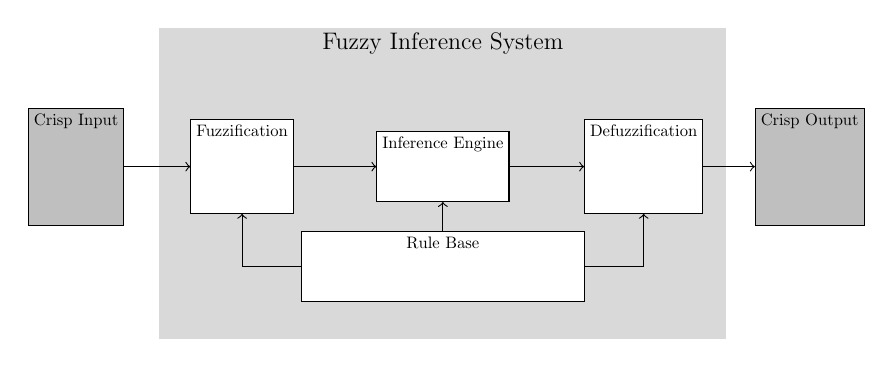
\begin{tikzpicture}[scale=0.6, transform shape]
    \node[fill=gray!30,text depth = 6cm,minimum width=12cm,font=\Large] (main){Fuzzy Inference System};
    \node[draw,fill=white!30, text depth=1cm] at ([yshift=1em]main.center)(infer){Inference Engine};
    \node[draw,fill=white!30, text depth=1cm, minimum width=6cm] at ([yshift=-5em]main.center)(rb){Rule Base};
    \node[draw,fill=white!30, text depth=1.5cm] at ([xshift=5em, yshift=1em]main.west)(fuzz){Fuzzification};
    \node[draw,fill=white!30, text depth=1.5cm] at ([xshift=-5em, yshift=1em]main.east)(defuzz){Defuzzification};
    \node[draw,fill=gray!50, text depth=2cm] at ([xshift=-5em, yshift=1em]main.west)(inp){Crisp Input};
    \node[draw,fill=gray!50, text depth=2cm] at ([xshift=5em, yshift=1em]main.east)(outp){Crisp Output};

    \node at ([xshift=5em, yshift=-5em]main.west)(ghostleft){};
    \node at ([xshift=-5em, yshift=-5em]main.east)(ghostright){};

    \draw[->](inp.east) -- (fuzz.west);
    \draw[->](fuzz.east) -- (infer.west);
    \draw[->](infer.east) -- (defuzz.west);
    \draw[->](defuzz.east) -- (outp.west);
    \draw[->](rb.north) -- (infer.south);
    \draw[->](rb.west) -- (ghostleft.center) -- (fuzz.south);
    \draw[->](rb.east) -- (ghostright.center) -- (defuzz.south);
\end{tikzpicture}

\end{frame}

\begin{frame}{Fuzzy Logic (3/5)}
    \centering
    Traditional vs. Fuzzy logic
    \begin{columns}
        \begin{column}{0.5\textwidth}
            \scalebox{0.45}{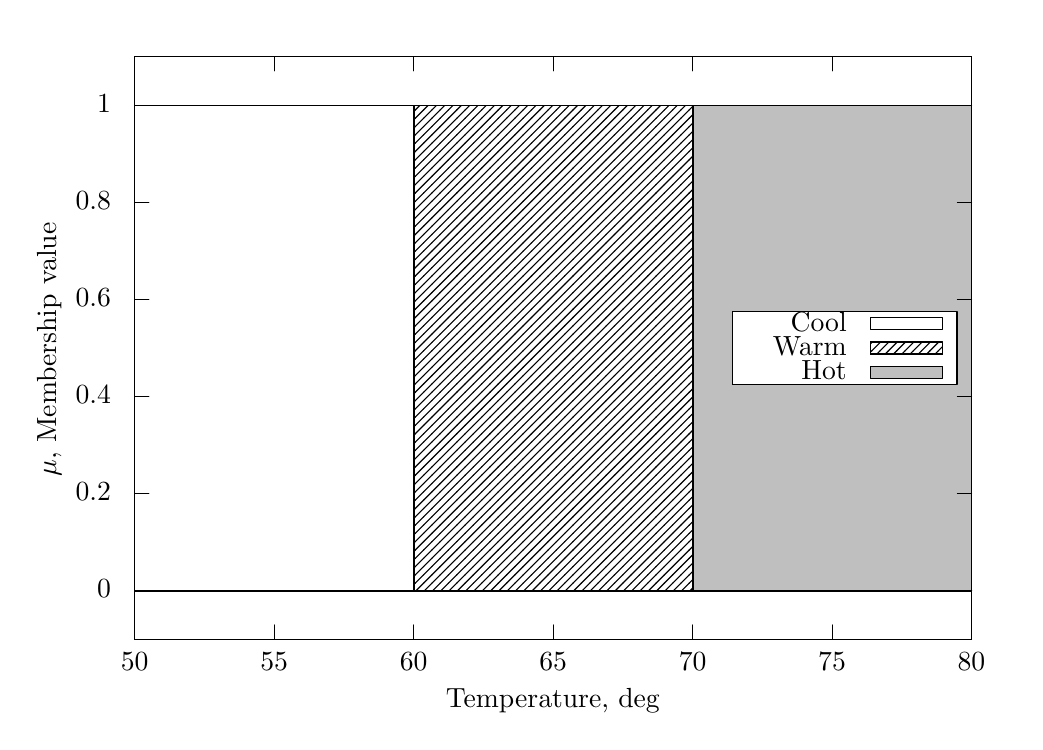
\begin{tikzpicture}[gnuplot]
%% generated with GNUPLOT 5.0p3 (Lua 5.1; terminal rev. 99, script rev. 100)
%% Thu 29 Mar 2018 12:26:43 AM EDT
\gpmonochromelines
\path (0.000,0.000) rectangle (12.500,8.750);
\gpcolor{color=gp lt color border}
\gpsetlinetype{gp lt border}
\gpsetdashtype{gp dt solid}
\gpsetlinewidth{1.00}
\draw[gp path] (1.320,1.601)--(1.500,1.601);
\draw[gp path] (11.947,1.601)--(11.767,1.601);
\node[gp node right] at (1.136,1.601) {$0$};
\draw[gp path] (1.320,2.834)--(1.500,2.834);
\draw[gp path] (11.947,2.834)--(11.767,2.834);
\node[gp node right] at (1.136,2.834) {$0.2$};
\draw[gp path] (1.320,4.067)--(1.500,4.067);
\draw[gp path] (11.947,4.067)--(11.767,4.067);
\node[gp node right] at (1.136,4.067) {$0.4$};
\draw[gp path] (1.320,5.299)--(1.500,5.299);
\draw[gp path] (11.947,5.299)--(11.767,5.299);
\node[gp node right] at (1.136,5.299) {$0.6$};
\draw[gp path] (1.320,6.532)--(1.500,6.532);
\draw[gp path] (11.947,6.532)--(11.767,6.532);
\node[gp node right] at (1.136,6.532) {$0.8$};
\draw[gp path] (1.320,7.765)--(1.500,7.765);
\draw[gp path] (11.947,7.765)--(11.767,7.765);
\node[gp node right] at (1.136,7.765) {$1$};
\draw[gp path] (1.320,0.985)--(1.320,1.165);
\draw[gp path] (1.320,8.381)--(1.320,8.201);
\node[gp node center] at (1.320,0.677) {$50$};
\draw[gp path] (3.091,0.985)--(3.091,1.165);
\draw[gp path] (3.091,8.381)--(3.091,8.201);
\node[gp node center] at (3.091,0.677) {$55$};
\draw[gp path] (4.862,0.985)--(4.862,1.165);
\draw[gp path] (4.862,8.381)--(4.862,8.201);
\node[gp node center] at (4.862,0.677) {$60$};
\draw[gp path] (6.634,0.985)--(6.634,1.165);
\draw[gp path] (6.634,8.381)--(6.634,8.201);
\node[gp node center] at (6.634,0.677) {$65$};
\draw[gp path] (8.405,0.985)--(8.405,1.165);
\draw[gp path] (8.405,8.381)--(8.405,8.201);
\node[gp node center] at (8.405,0.677) {$70$};
\draw[gp path] (10.176,0.985)--(10.176,1.165);
\draw[gp path] (10.176,8.381)--(10.176,8.201);
\node[gp node center] at (10.176,0.677) {$75$};
\draw[gp path] (11.947,0.985)--(11.947,1.165);
\draw[gp path] (11.947,8.381)--(11.947,8.201);
\node[gp node center] at (11.947,0.677) {$80$};
\draw[gp path] (1.320,8.381)--(1.320,0.985)--(11.947,0.985)--(11.947,8.381)--cycle;
\node[gp node center,rotate=-270] at (0.246,4.683) {$\mu$, Membership value};
\node[gp node center] at (6.633,0.215) {Temperature, $\deg$};
\draw[gp path] (8.915,4.221)--(8.915,5.145)--(11.763,5.145)--(11.763,4.221)--cycle;
\gpfill{color=gp lt color border,gp pattern 0,pattern color=.} (1.320,7.765)--(4.862,7.765)--(4.862,1.601)--(8.405,1.601)%
    --(8.405,1.601)--(11.947,1.601)--(11.947,1.601)--cycle;
\draw[gp path] (1.320,7.765)--(4.862,7.765)--(4.862,1.601)--(8.405,1.601)--(11.947,1.601);
\gpfill{color=gp lt color border,gp pattern 1,pattern color=.} (1.320,1.601)--(4.862,1.601)--(4.862,7.765)--(8.405,7.765)%
    --(8.405,1.601)--(11.947,1.601)--(11.947,1.601)--cycle;
\gpsetdashtype{gp dt 2}
\draw[gp path] (1.320,1.601)--(4.862,1.601)--(4.862,7.765)--(8.405,7.765)--(8.405,1.601)%
  --(11.947,1.601);
\gpfill{color=gp lt color border,opacity=0.25} (1.320,1.601)--(4.862,1.601)--(4.862,1.601)--(8.405,1.601)%
    --(8.405,7.765)--(11.947,7.765)--(11.947,1.601)--cycle;
\gpsetdashtype{gp dt 3}
\draw[gp path] (1.320,1.601)--(4.862,1.601)--(8.405,1.601)--(8.405,7.765)--(11.947,7.765)%
  --(11.947,1.601);
\gpfill{color=gpbgfillcolor} (8.915,4.221)--(11.763,4.221)--(11.763,5.145)--(8.915,5.145)--cycle;
\gpsetdashtype{gp dt solid}
\draw[gp path] (8.915,4.221)--(8.915,5.145)--(11.763,5.145)--(11.763,4.221)--cycle;
\node[gp node right] at (10.479,4.991) {Cool};
\gpfill{color=gp lt color border,gp pattern 0,pattern color=.} (10.663,4.914)--(11.579,4.914)--(11.579,5.068)--(10.663,5.068)--cycle;
\draw[gp path] (10.663,4.914)--(11.579,4.914)--(11.579,5.068)--(10.663,5.068)--cycle;
\node[gp node right] at (10.479,4.683) {Warm};
\gpfill{color=gp lt color border,gp pattern 1,pattern color=.} (10.663,4.606)--(11.579,4.606)--(11.579,4.760)--(10.663,4.760)--cycle;
\gpsetdashtype{gp dt 2}
\draw[gp path] (10.663,4.606)--(11.579,4.606)--(11.579,4.760)--(10.663,4.760)--cycle;
\node[gp node right] at (10.479,4.375) {Hot};
\gpfill{color=gp lt color border,opacity=0.25} (10.663,4.298)--(11.579,4.298)--(11.579,4.452)--(10.663,4.452)--cycle;
\gpsetdashtype{gp dt 3}
\draw[gp path] (10.663,4.298)--(11.579,4.298)--(11.579,4.452)--(10.663,4.452)--cycle;
\gpsetdashtype{gp dt solid}
\draw[gp path] (1.320,8.381)--(1.320,0.985)--(11.947,0.985)--(11.947,8.381)--cycle;
%% coordinates of the plot area
\gpdefrectangularnode{gp plot 1}{\pgfpoint{1.320cm}{0.985cm}}{\pgfpoint{11.947cm}{8.381cm}}
\end{tikzpicture}
%% gnuplot variables
}
        \end{column}
        \begin{column}{0.5\textwidth}
            \scalebox{0.45}{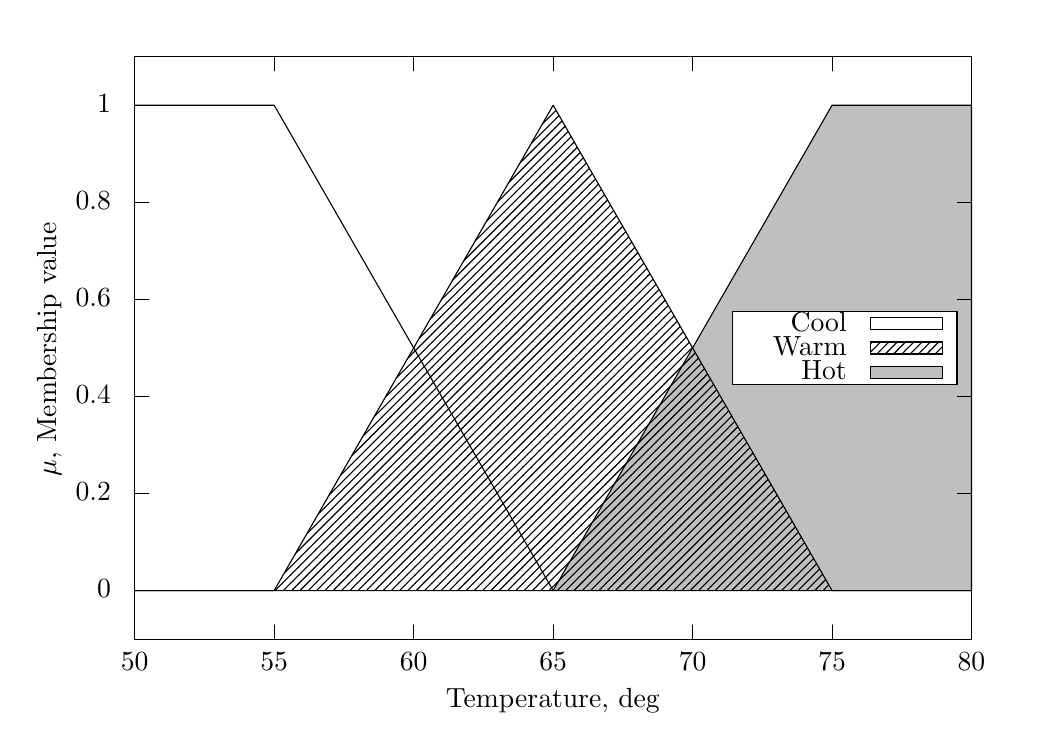
\begin{tikzpicture}[gnuplot]
%% generated with GNUPLOT 5.0p3 (Lua 5.1; terminal rev. 99, script rev. 100)
%% Thu 29 Mar 2018 12:26:43 AM EDT
\gpmonochromelines
\path (0.000,0.000) rectangle (12.500,8.750);
\gpcolor{color=gp lt color border}
\gpsetlinetype{gp lt border}
\gpsetdashtype{gp dt solid}
\gpsetlinewidth{1.00}
\draw[gp path] (1.320,1.601)--(1.500,1.601);
\draw[gp path] (11.947,1.601)--(11.767,1.601);
\node[gp node right] at (1.136,1.601) {$0$};
\draw[gp path] (1.320,2.834)--(1.500,2.834);
\draw[gp path] (11.947,2.834)--(11.767,2.834);
\node[gp node right] at (1.136,2.834) {$0.2$};
\draw[gp path] (1.320,4.067)--(1.500,4.067);
\draw[gp path] (11.947,4.067)--(11.767,4.067);
\node[gp node right] at (1.136,4.067) {$0.4$};
\draw[gp path] (1.320,5.299)--(1.500,5.299);
\draw[gp path] (11.947,5.299)--(11.767,5.299);
\node[gp node right] at (1.136,5.299) {$0.6$};
\draw[gp path] (1.320,6.532)--(1.500,6.532);
\draw[gp path] (11.947,6.532)--(11.767,6.532);
\node[gp node right] at (1.136,6.532) {$0.8$};
\draw[gp path] (1.320,7.765)--(1.500,7.765);
\draw[gp path] (11.947,7.765)--(11.767,7.765);
\node[gp node right] at (1.136,7.765) {$1$};
\draw[gp path] (1.320,0.985)--(1.320,1.165);
\draw[gp path] (1.320,8.381)--(1.320,8.201);
\node[gp node center] at (1.320,0.677) {$50$};
\draw[gp path] (3.091,0.985)--(3.091,1.165);
\draw[gp path] (3.091,8.381)--(3.091,8.201);
\node[gp node center] at (3.091,0.677) {$55$};
\draw[gp path] (4.862,0.985)--(4.862,1.165);
\draw[gp path] (4.862,8.381)--(4.862,8.201);
\node[gp node center] at (4.862,0.677) {$60$};
\draw[gp path] (6.634,0.985)--(6.634,1.165);
\draw[gp path] (6.634,8.381)--(6.634,8.201);
\node[gp node center] at (6.634,0.677) {$65$};
\draw[gp path] (8.405,0.985)--(8.405,1.165);
\draw[gp path] (8.405,8.381)--(8.405,8.201);
\node[gp node center] at (8.405,0.677) {$70$};
\draw[gp path] (10.176,0.985)--(10.176,1.165);
\draw[gp path] (10.176,8.381)--(10.176,8.201);
\node[gp node center] at (10.176,0.677) {$75$};
\draw[gp path] (11.947,0.985)--(11.947,1.165);
\draw[gp path] (11.947,8.381)--(11.947,8.201);
\node[gp node center] at (11.947,0.677) {$80$};
\draw[gp path] (1.320,8.381)--(1.320,0.985)--(11.947,0.985)--(11.947,8.381)--cycle;
\node[gp node center,rotate=-270] at (0.246,4.683) {$\mu$, Membership value};
\node[gp node center] at (6.633,0.215) {Temperature, $\deg$};
\draw[gp path] (8.915,4.221)--(8.915,5.145)--(11.763,5.145)--(11.763,4.221)--cycle;
\gpfill{color=gp lt color border,gp pattern 0,pattern color=.} (1.320,7.765)--(3.091,7.765)--(6.634,1.601)--(10.176,1.601)%
    --(11.947,1.601)--(11.947,1.601)--cycle;
\draw[gp path] (1.320,7.765)--(3.091,7.765)--(6.634,1.601)--(10.176,1.601)--(11.947,1.601);
\gpfill{color=gp lt color border,gp pattern 1,pattern color=.} (1.320,1.601)--(3.091,1.601)--(6.634,7.765)--(10.176,1.601)%
    --(11.947,1.601)--(11.947,1.601)--cycle;
\gpsetdashtype{gp dt 2}
\draw[gp path] (1.320,1.601)--(3.091,1.601)--(6.634,7.765)--(10.176,1.601)--(11.947,1.601);
\gpfill{color=gp lt color border,opacity=0.25} (1.320,1.601)--(3.091,1.601)--(6.634,1.601)--(10.176,7.765)%
    --(11.947,7.765)--(11.947,1.601)--cycle;
\gpsetdashtype{gp dt 3}
\draw[gp path] (1.320,1.601)--(3.091,1.601)--(6.634,1.601)--(10.176,7.765)--(11.947,7.765)%
  --(11.947,1.601);
\gpfill{color=gpbgfillcolor} (8.915,4.221)--(11.763,4.221)--(11.763,5.145)--(8.915,5.145)--cycle;
\gpsetdashtype{gp dt solid}
\draw[gp path] (8.915,4.221)--(8.915,5.145)--(11.763,5.145)--(11.763,4.221)--cycle;
\node[gp node right] at (10.479,4.991) {Cool};
\gpfill{color=gp lt color border,gp pattern 0,pattern color=.} (10.663,4.914)--(11.579,4.914)--(11.579,5.068)--(10.663,5.068)--cycle;
\draw[gp path] (10.663,4.914)--(11.579,4.914)--(11.579,5.068)--(10.663,5.068)--cycle;
\node[gp node right] at (10.479,4.683) {Warm};
\gpfill{color=gp lt color border,gp pattern 1,pattern color=.} (10.663,4.606)--(11.579,4.606)--(11.579,4.760)--(10.663,4.760)--cycle;
\gpsetdashtype{gp dt 2}
\draw[gp path] (10.663,4.606)--(11.579,4.606)--(11.579,4.760)--(10.663,4.760)--cycle;
\node[gp node right] at (10.479,4.375) {Hot};
\gpfill{color=gp lt color border,opacity=0.25} (10.663,4.298)--(11.579,4.298)--(11.579,4.452)--(10.663,4.452)--cycle;
\gpsetdashtype{gp dt 3}
\draw[gp path] (10.663,4.298)--(11.579,4.298)--(11.579,4.452)--(10.663,4.452)--cycle;
\gpsetdashtype{gp dt solid}
\draw[gp path] (1.320,8.381)--(1.320,0.985)--(11.947,0.985)--(11.947,8.381)--cycle;
%% coordinates of the plot area
\gpdefrectangularnode{gp plot 1}{\pgfpoint{1.320cm}{0.985cm}}{\pgfpoint{11.947cm}{8.381cm}}
\end{tikzpicture}
%% gnuplot variables
}
        \end{column}
    \end{columns}
\end{frame}

\begin{frame}{Fuzzy Logic (4/5)}
    \centering
    Defuzzification\\
    \scalebox{0.6}{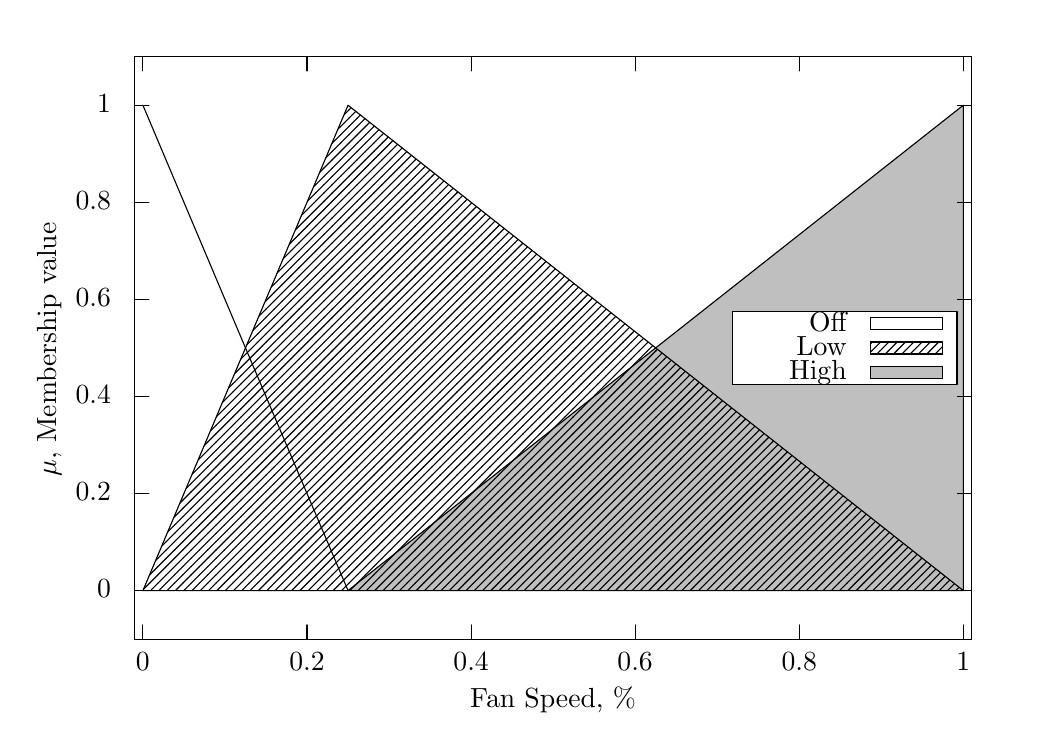
\begin{tikzpicture}[gnuplot]
%% generated with GNUPLOT 5.0p3 (Lua 5.1; terminal rev. 99, script rev. 100)
%% Thu 29 Mar 2018 12:26:43 AM EDT
\gpmonochromelines
\path (0.000,0.000) rectangle (12.500,8.750);
\gpcolor{color=gp lt color border}
\gpsetlinetype{gp lt border}
\gpsetdashtype{gp dt solid}
\gpsetlinewidth{1.00}
\draw[gp path] (1.320,1.601)--(1.500,1.601);
\draw[gp path] (11.947,1.601)--(11.767,1.601);
\node[gp node right] at (1.136,1.601) {$0$};
\draw[gp path] (1.320,2.834)--(1.500,2.834);
\draw[gp path] (11.947,2.834)--(11.767,2.834);
\node[gp node right] at (1.136,2.834) {$0.2$};
\draw[gp path] (1.320,4.067)--(1.500,4.067);
\draw[gp path] (11.947,4.067)--(11.767,4.067);
\node[gp node right] at (1.136,4.067) {$0.4$};
\draw[gp path] (1.320,5.299)--(1.500,5.299);
\draw[gp path] (11.947,5.299)--(11.767,5.299);
\node[gp node right] at (1.136,5.299) {$0.6$};
\draw[gp path] (1.320,6.532)--(1.500,6.532);
\draw[gp path] (11.947,6.532)--(11.767,6.532);
\node[gp node right] at (1.136,6.532) {$0.8$};
\draw[gp path] (1.320,7.765)--(1.500,7.765);
\draw[gp path] (11.947,7.765)--(11.767,7.765);
\node[gp node right] at (1.136,7.765) {$1$};
\draw[gp path] (1.424,0.985)--(1.424,1.165);
\draw[gp path] (1.424,8.381)--(1.424,8.201);
\node[gp node center] at (1.424,0.677) {$0$};
\draw[gp path] (3.508,0.985)--(3.508,1.165);
\draw[gp path] (3.508,8.381)--(3.508,8.201);
\node[gp node center] at (3.508,0.677) {$0.2$};
\draw[gp path] (5.592,0.985)--(5.592,1.165);
\draw[gp path] (5.592,8.381)--(5.592,8.201);
\node[gp node center] at (5.592,0.677) {$0.4$};
\draw[gp path] (7.675,0.985)--(7.675,1.165);
\draw[gp path] (7.675,8.381)--(7.675,8.201);
\node[gp node center] at (7.675,0.677) {$0.6$};
\draw[gp path] (9.759,0.985)--(9.759,1.165);
\draw[gp path] (9.759,8.381)--(9.759,8.201);
\node[gp node center] at (9.759,0.677) {$0.8$};
\draw[gp path] (11.843,0.985)--(11.843,1.165);
\draw[gp path] (11.843,8.381)--(11.843,8.201);
\node[gp node center] at (11.843,0.677) {$1$};
\draw[gp path] (1.320,8.381)--(1.320,0.985)--(11.947,0.985)--(11.947,8.381)--cycle;
\node[gp node center,rotate=-270] at (0.246,4.683) {$\mu$, Membership value};
\node[gp node center] at (6.633,0.215) {Fan Speed, $\%$};
\draw[gp path] (8.915,4.221)--(8.915,5.145)--(11.763,5.145)--(11.763,4.221)--cycle;
\gpfill{color=gp lt color border,gp pattern 0,pattern color=.} (1.424,7.765)--(4.029,1.601)--(11.843,1.601)--(11.843,1.601)--cycle;
\draw[gp path] (1.424,7.765)--(4.029,1.601)--(11.843,1.601);
\gpfill{color=gp lt color border,gp pattern 1,pattern color=.} (1.424,1.601)--(4.029,7.765)--(11.843,1.601)--(11.843,1.601)--cycle;
\gpsetdashtype{gp dt 2}
\draw[gp path] (1.424,1.601)--(4.029,7.765)--(11.843,1.601);
\gpfill{color=gp lt color border,opacity=0.25} (1.424,1.601)--(4.029,1.601)--(11.843,7.765)--(11.843,1.601)--cycle;
\gpsetdashtype{gp dt 3}
\draw[gp path] (1.424,1.601)--(4.029,1.601)--(11.843,7.765)--(11.843,1.601);
\gpfill{color=gpbgfillcolor} (8.915,4.221)--(11.763,4.221)--(11.763,5.145)--(8.915,5.145)--cycle;
\gpsetdashtype{gp dt solid}
\draw[gp path] (8.915,4.221)--(8.915,5.145)--(11.763,5.145)--(11.763,4.221)--cycle;
\node[gp node right] at (10.479,4.991) {Off};
\gpfill{color=gp lt color border,gp pattern 0,pattern color=.} (10.663,4.914)--(11.579,4.914)--(11.579,5.068)--(10.663,5.068)--cycle;
\draw[gp path] (10.663,4.914)--(11.579,4.914)--(11.579,5.068)--(10.663,5.068)--cycle;
\node[gp node right] at (10.479,4.683) {Low};
\gpfill{color=gp lt color border,gp pattern 1,pattern color=.} (10.663,4.606)--(11.579,4.606)--(11.579,4.760)--(10.663,4.760)--cycle;
\gpsetdashtype{gp dt 2}
\draw[gp path] (10.663,4.606)--(11.579,4.606)--(11.579,4.760)--(10.663,4.760)--cycle;
\node[gp node right] at (10.479,4.375) {High};
\gpfill{color=gp lt color border,opacity=0.25} (10.663,4.298)--(11.579,4.298)--(11.579,4.452)--(10.663,4.452)--cycle;
\gpsetdashtype{gp dt 3}
\draw[gp path] (10.663,4.298)--(11.579,4.298)--(11.579,4.452)--(10.663,4.452)--cycle;
\gpsetdashtype{gp dt solid}
\draw[gp path] (1.320,8.381)--(1.320,0.985)--(11.947,0.985)--(11.947,8.381)--cycle;
%% coordinates of the plot area
\gpdefrectangularnode{gp plot 1}{\pgfpoint{1.320cm}{0.985cm}}{\pgfpoint{11.947cm}{8.381cm}}
\end{tikzpicture}
%% gnuplot variables
}
\end{frame}

\begin{frame}{Fuzzy Logic (5/5)}
    \vspace{2em}
    \begin{tabular}{cccccc}
        IF &  \emph{temperature} is & COOL, & THEN & \emph{fan speed} is & OFF\\
        IF &  \emph{temperature} is & WARM, & THEN & \emph{fan speed} is & LOW\\
        IF &  \emph{temperature} is & HOT,  & THEN & \emph{fan speed} is & HIGH
    \end{tabular}\vspace{1em}
    \centering
    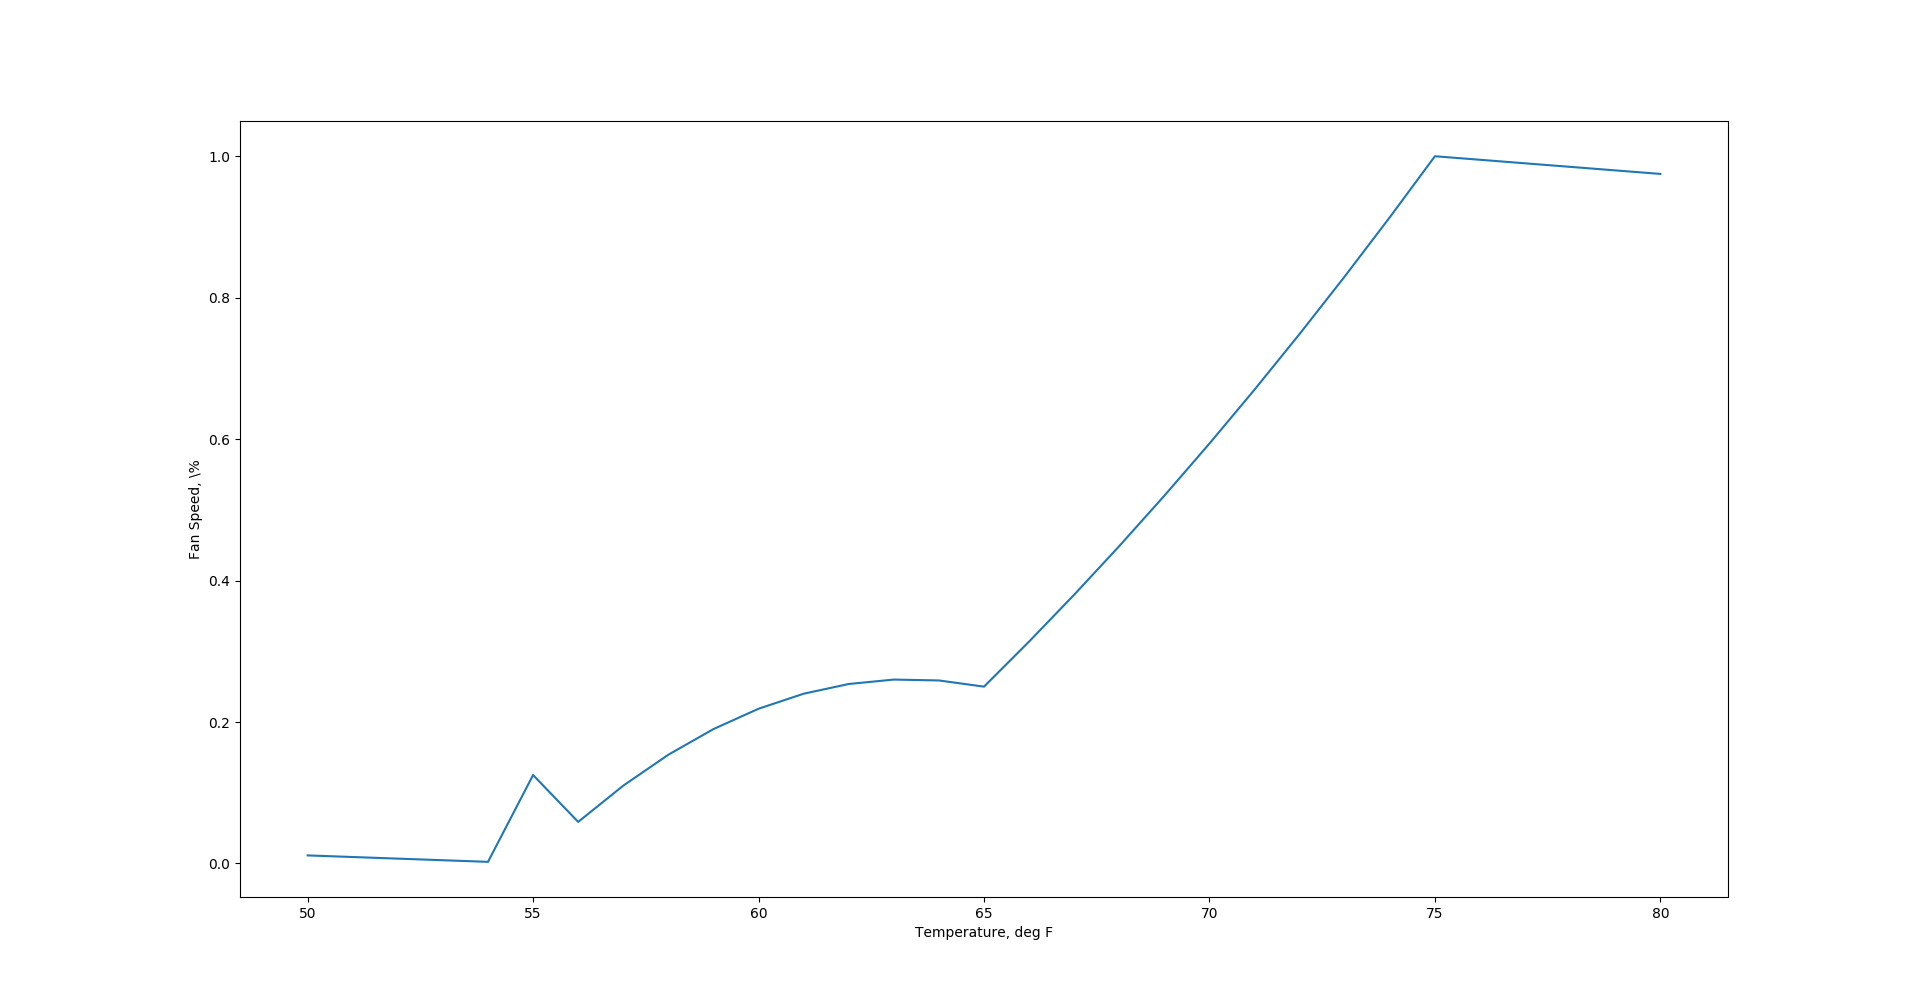
\includegraphics[width=0.8\textwidth]{../images/fuzzyfan}
\end{frame}


\subsection{Genetic Algorithms}
\begin{frame}{Genetic Algorithm}
\begin{itemize}
\item To solve a problem with a GA you need:
    \begin{itemize}
    \item A way to encode a solution as a genetic unit (chromosome)
    \item A way to create an initial population of candidates
    \item A grading or cost function to assess individual fitness
    \begin{itemize}
        \item We are trying for ``survival of the fittest'', but what ``fit'' means is up to us
    \end{itemize}
    \item Genetic operators
    \item General guidelines for the mechanics of the GA
    \begin{itemize}
        \item How many individuals make up a population
        \item How many generations until we stop looking
        \item How do we apply the genetic operators to each population
    \end{itemize}
    \end{itemize}
\end{itemize}
\end{frame}

\begin{frame}{GA Operational Flow}
\tikz[overlay] \node [at=(current page.center)] {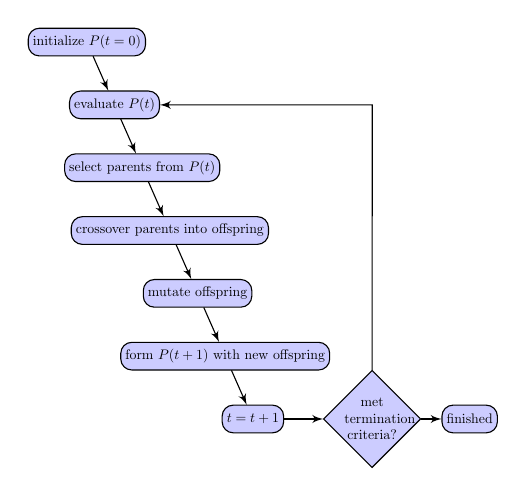
\begin{tikzpicture}[node distance=25pt and 15pt, auto, scale = 0.5, transform shape]
\node[draw, block] (init){initialize $P(t=0)$};
\node[draw, block, below = of init, xshift=2em](eval){evaluate $P(t)$};
\node[draw, block, below = of eval, xshift=2em](select){select parents from $P(t)$};
\node[draw, block, below = of select, xshift=2em](cross){crossover parents into offspring};
\node[draw, block, below = of cross, xshift=2em](mut){mutate offspring};
\node[draw, block, below = of mut, xshift=2em](ass){form $P(t+1)$ with new offspring};
\node[draw, block, below = of ass, xshift=2em](iter){$t=t+1$};
\node[draw, decision, right= of iter](term){met\\termination criteria?};
\node[draw, block, right= of term](fin){finished};

\node [right= of eval, xshift=13.5em](dummy1){};

\draw[line](init) -- (eval);
\draw[line](eval) -- (select);
\draw[line](select) -- (cross);
\draw[line](cross) -- (mut);
\draw[line](mut) -- (ass);
\draw[line](ass) --coordinate[midway](bisect) (iter);
\draw[line](iter) -- (term);
\draw[line](term) -- (fin);
\draw[line](term.north) -- (dummy1.center) -- (eval);
\end{tikzpicture}
};
\end{frame}

\begin{frame}{Chromosomal Representation}
    \begin{itemize}
        \item Careful to obtain good mapping from phenotype to genotype 
        \item For this work, most FISs are encoded with a mix of real values and discrete integers
        \item The fuzzy fan controller:
            \begin{itemize}
                \item \begin{math}
                        \left(0, 0, 55, 65\right) \left(55, 65, 75\right) \left(65, 75, 100, 100\right)
                    \end{math}
                    \begin{math}
                        |\left(0, 0, 0.25\right) \left(0, 0.25, 1\right) \left(0.25, 1, 1\right)
                    \end{math}
                    \begin{math}
                        \left[0, 1, 2\right]
                    \end{math}
            \end{itemize}
    \end{itemize}
\end{frame}


%\begin{frame}{Fitness Function}
%\tikz[overlay] \node [at=(current page.center)] {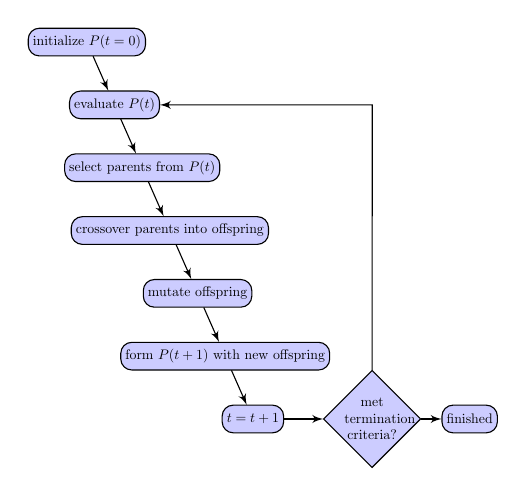
\begin{tikzpicture}[node distance=25pt and 15pt, auto, scale = 0.5, transform shape]
\node[draw, block] (init){initialize $P(t=0)$};
\node[draw, block, below = of init, xshift=2em](eval){evaluate $P(t)$};
\node[draw, block, below = of eval, xshift=2em](select){select parents from $P(t)$};
\node[draw, block, below = of select, xshift=2em](cross){crossover parents into offspring};
\node[draw, block, below = of cross, xshift=2em](mut){mutate offspring};
\node[draw, block, below = of mut, xshift=2em](ass){form $P(t+1)$ with new offspring};
\node[draw, block, below = of ass, xshift=2em](iter){$t=t+1$};
\node[draw, decision, right= of iter](term){met\\termination criteria?};
\node[draw, block, right= of term](fin){finished};

\node [right= of eval, xshift=13.5em](dummy1){};

\draw[line](init) -- (eval);
\draw[line](eval) -- (select);
\draw[line](select) -- (cross);
\draw[line](cross) -- (mut);
\draw[line](mut) -- (ass);
\draw[line](ass) --coordinate[midway](bisect) (iter);
\draw[line](iter) -- (term);
\draw[line](term) -- (fin);
\draw[line](term.north) -- (dummy1.center) -- (eval);
\end{tikzpicture}
};
%\tikz[overlay] \draw[red,thick] (eval) ellipse (1.25 and 0.4);
%\end{frame}

%\begin{frame}{Fitness Function}
%Choosing a fitness function
%\begin{itemize}
%\item Function optimization
    %\begin{itemize}
    %\item Simply try to maximize (or minimize, in the case of cost function)
    %\end{itemize}
%\item Line fitting
    %\begin{itemize}
    %\item Least means square
    %\end{itemize}
%\item Control Response
    %\begin{itemize}
    %\item Penalize bad behavior (overshoot, vibration)
    %\item Encourage good traits (settling time, minimal error)
    %\end{itemize}
%\item A bad cost function will produce a bad result
%\end{itemize}
%\end{frame}

%\subsection{Selection Mechanism}
\begin{frame}{Selection}
\tikz[overlay] \node [at=(current page.center)] {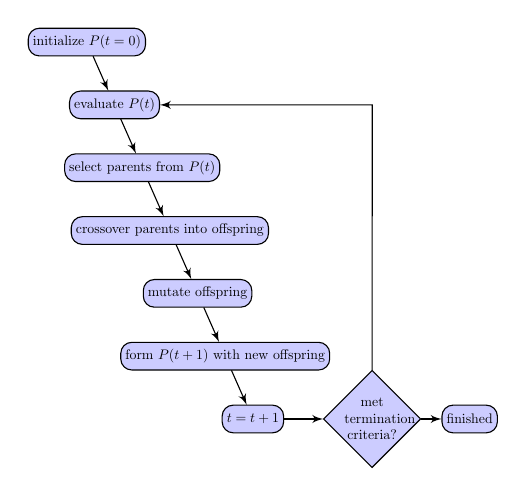
\begin{tikzpicture}[node distance=25pt and 15pt, auto, scale = 0.5, transform shape]
\node[draw, block] (init){initialize $P(t=0)$};
\node[draw, block, below = of init, xshift=2em](eval){evaluate $P(t)$};
\node[draw, block, below = of eval, xshift=2em](select){select parents from $P(t)$};
\node[draw, block, below = of select, xshift=2em](cross){crossover parents into offspring};
\node[draw, block, below = of cross, xshift=2em](mut){mutate offspring};
\node[draw, block, below = of mut, xshift=2em](ass){form $P(t+1)$ with new offspring};
\node[draw, block, below = of ass, xshift=2em](iter){$t=t+1$};
\node[draw, decision, right= of iter](term){met\\termination criteria?};
\node[draw, block, right= of term](fin){finished};

\node [right= of eval, xshift=13.5em](dummy1){};

\draw[line](init) -- (eval);
\draw[line](eval) -- (select);
\draw[line](select) -- (cross);
\draw[line](cross) -- (mut);
\draw[line](mut) -- (ass);
\draw[line](ass) --coordinate[midway](bisect) (iter);
\draw[line](iter) -- (term);
\draw[line](term) -- (fin);
\draw[line](term.north) -- (dummy1.center) -- (eval);
\end{tikzpicture}
};
\tikz[overlay] \draw[red,thick] (select) ellipse (2 and 0.4);
\end{frame}

\begin{frame}{Selection Mechanism}
    \vspace{1em}
    \begin{itemize}
        \item Want to retain good genes in future generations
        \item Favor fitter (harder, better, faster, stronger) parents to reproduce
        \item Main method used in this work is a triangular probability distribution
    \end{itemize}
    \centering
    \scalebox{0.7}{
        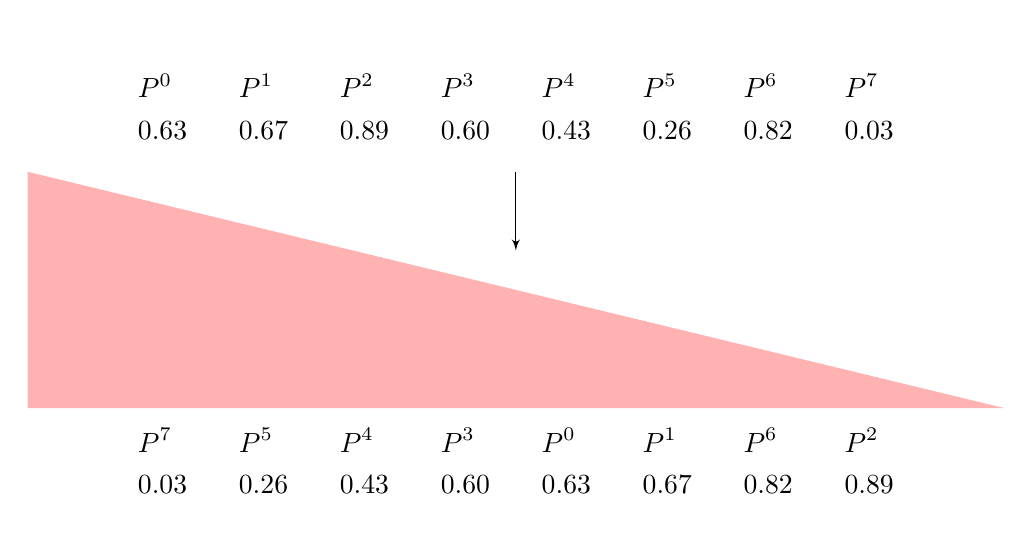
\begin{tikzpicture}
    \draw[fill=red!30, draw=none](-6.2,-1) -- (6.2,-4) -- (-6.2,-4) -- cycle;
    \node(presort){
            \begin{minipage}{0.9\textwidth}
                \begin{align*}
                    &P^{0}&&P^{1}&&P^{2}&&P^{3}&&P^{4}&&P^{5}&&P^{6}&&P^{7}\\
                    &0.63&&0.67&&0.89&&0.60&&0.43&&0.26&&0.82&&0.03
                \end{align*}
            \end{minipage}
        };
    \node[below of= presort, yshift=-3.5cm] (sorted){
            \begin{minipage}{0.9\textwidth}
                \begin{align*}
                    &P^{7}&&P^{5}&&P^{4}&&P^{3}&&P^{0}&&P^{1}&&P^{6}&&P^{2}\\
                    &0.03&&0.26&&0.43&&0.60&&0.63&&0.67&&0.82&&0.89
                \end{align*}
            \end{minipage}
        };
    \draw[line](0,-1) -- (0,-2);

\end{tikzpicture}




    }
\end{frame}

%\subsection{Genetic Operators}
%\subsubsection{Crossover}
\usebackgroundtemplate{}
\begin{frame}{Crossover/Mating}
\tikz[overlay] \node [at=(current page.center)] {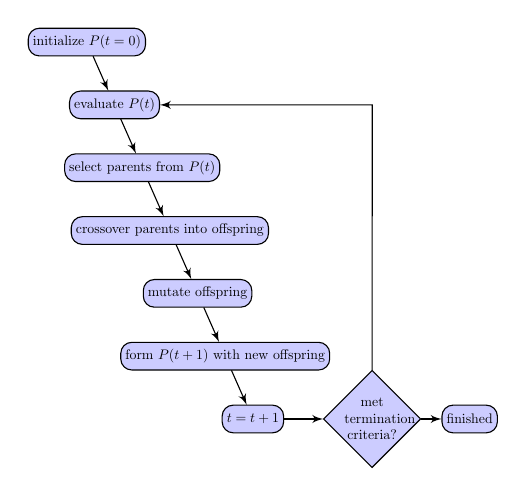
\begin{tikzpicture}[node distance=25pt and 15pt, auto, scale = 0.5, transform shape]
\node[draw, block] (init){initialize $P(t=0)$};
\node[draw, block, below = of init, xshift=2em](eval){evaluate $P(t)$};
\node[draw, block, below = of eval, xshift=2em](select){select parents from $P(t)$};
\node[draw, block, below = of select, xshift=2em](cross){crossover parents into offspring};
\node[draw, block, below = of cross, xshift=2em](mut){mutate offspring};
\node[draw, block, below = of mut, xshift=2em](ass){form $P(t+1)$ with new offspring};
\node[draw, block, below = of ass, xshift=2em](iter){$t=t+1$};
\node[draw, decision, right= of iter](term){met\\termination criteria?};
\node[draw, block, right= of term](fin){finished};

\node [right= of eval, xshift=13.5em](dummy1){};

\draw[line](init) -- (eval);
\draw[line](eval) -- (select);
\draw[line](select) -- (cross);
\draw[line](cross) -- (mut);
\draw[line](mut) -- (ass);
\draw[line](ass) --coordinate[midway](bisect) (iter);
\draw[line](iter) -- (term);
\draw[line](term) -- (fin);
\draw[line](term.north) -- (dummy1.center) -- (eval);
\end{tikzpicture}
};
\tikz[overlay] \draw[red,thick] (cross) ellipse (2.5 and 0.4);
\end{frame}

\begin{frame}{Crossover/Mating}
Operators depend on the method of encoding
\begin{itemize}
\item Binary Encoded Chromosomes
    \begin{itemize}
    \item\only<1>{Single/Double/Multi Point Crossover}
    \only<2-> {Single/Double/Multi Point Crossover \(\checkmark\)}
    \item\only<1-2>{ Hamming cliff }
    \only<3-> {Hamming cliff\(\times\)}
    \item\only<1-3> {Representation does not reflect solution space}
    \only<4-> {Representation does not reflect solution space\(\times\)}
    \end{itemize}
\item Real-Valued Genetic Encoding
    \begin{itemize}
    \item \only<1-4>{Simple/Flat/Blended Crossover}
    \only<5-> {Simple/Flat/Blended Crossover \(\checkmark\)}
    \item \only<1-5> {Recombination of parents in neighborhood}
    \only<6-> {Recombination of parents in neighborhood \(\checkmark\)}
    \item \only<1-6>{Often, chromosome represents actual solution -- no encoding necessary!}
    \only<7->{Often, chromosome represents actual solution -- no encoding necessary\(\checkmark\)}
    \end{itemize}
\item<7-> Recombination is the way in which the GA converges
\end{itemize}
\end{frame}

%\subsubsection{Mutation}
\usebackgroundtemplate{}
\begin{frame}{Mutation}
\tikz[overlay] \node [at=(current page.center)] {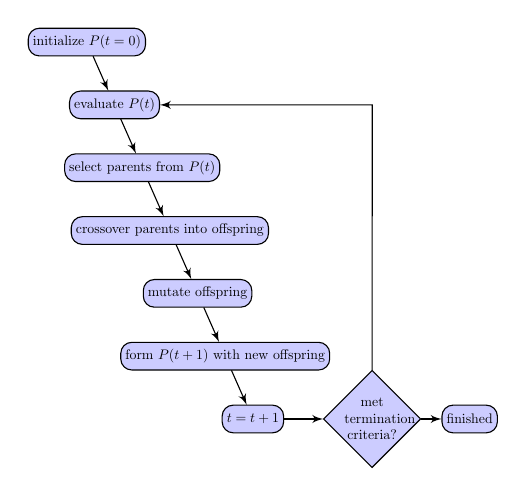
\begin{tikzpicture}[node distance=25pt and 15pt, auto, scale = 0.5, transform shape]
\node[draw, block] (init){initialize $P(t=0)$};
\node[draw, block, below = of init, xshift=2em](eval){evaluate $P(t)$};
\node[draw, block, below = of eval, xshift=2em](select){select parents from $P(t)$};
\node[draw, block, below = of select, xshift=2em](cross){crossover parents into offspring};
\node[draw, block, below = of cross, xshift=2em](mut){mutate offspring};
\node[draw, block, below = of mut, xshift=2em](ass){form $P(t+1)$ with new offspring};
\node[draw, block, below = of ass, xshift=2em](iter){$t=t+1$};
\node[draw, decision, right= of iter](term){met\\termination criteria?};
\node[draw, block, right= of term](fin){finished};

\node [right= of eval, xshift=13.5em](dummy1){};

\draw[line](init) -- (eval);
\draw[line](eval) -- (select);
\draw[line](select) -- (cross);
\draw[line](cross) -- (mut);
\draw[line](mut) -- (ass);
\draw[line](ass) --coordinate[midway](bisect) (iter);
\draw[line](iter) -- (term);
\draw[line](term) -- (fin);
\draw[line](term.north) -- (dummy1.center) -- (eval);
\end{tikzpicture}
};
\tikz[overlay] \draw[red,thick] (mut) ellipse (1.5 and 0.4);
\end{frame}

\begin{frame}{Mutation}
\begin{itemize}
\item Choose \(k\) number of genes to mutate
\item Randomly choose \(k\) genes in each chromosome which is being mutated and change them
\item[] Binary Encoding
    \begin{itemize}
    \item Flip the bit
    \end{itemize}
\item[] Real-Valued Encoding
    \begin{itemize}
    \item Random disturbance or random generation
    \item Sometimes advantageous to make it non-uniform with later generations
    \end{itemize}
\item Mutation is a factor which helps exploration of the solution space
\end{itemize}
\end{frame}

%\subsubsection{Iteration}
%\usebackgroundtemplate{}
%\begin{frame}{Iterate}
%\tikz[overlay] \node [at=(current page.center)] {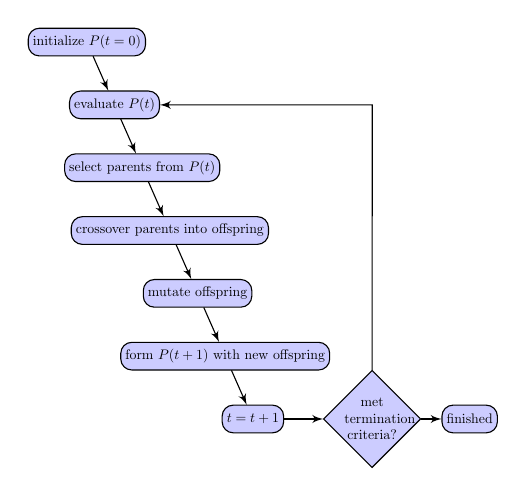
\begin{tikzpicture}[node distance=25pt and 15pt, auto, scale = 0.5, transform shape]
\node[draw, block] (init){initialize $P(t=0)$};
\node[draw, block, below = of init, xshift=2em](eval){evaluate $P(t)$};
\node[draw, block, below = of eval, xshift=2em](select){select parents from $P(t)$};
\node[draw, block, below = of select, xshift=2em](cross){crossover parents into offspring};
\node[draw, block, below = of cross, xshift=2em](mut){mutate offspring};
\node[draw, block, below = of mut, xshift=2em](ass){form $P(t+1)$ with new offspring};
\node[draw, block, below = of ass, xshift=2em](iter){$t=t+1$};
\node[draw, decision, right= of iter](term){met\\termination criteria?};
\node[draw, block, right= of term](fin){finished};

\node [right= of eval, xshift=13.5em](dummy1){};

\draw[line](init) -- (eval);
\draw[line](eval) -- (select);
\draw[line](select) -- (cross);
\draw[line](cross) -- (mut);
\draw[line](mut) -- (ass);
\draw[line](ass) --coordinate[midway](bisect) (iter);
\draw[line](iter) -- (term);
\draw[line](term) -- (fin);
\draw[line](term.north) -- (dummy1.center) -- (eval);
\end{tikzpicture}
};
%\tikz[overlay] \draw[red,thick] (bisect) ellipse (2.5 and 1);
%\end{frame}

%\subsubsection{Termination Criteria}
%\begin{frame}{Terminate}
%\tikz[overlay] \node [at=(current page.center)] {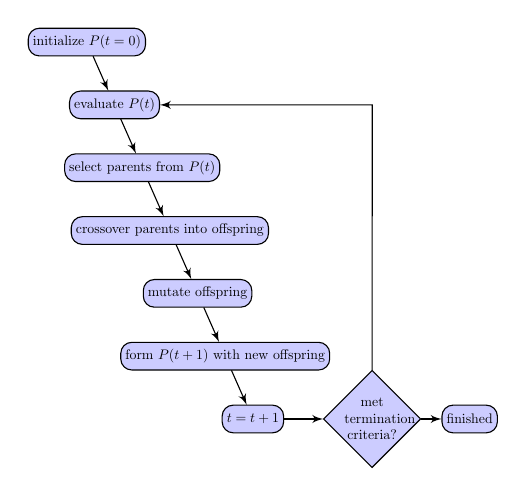
\begin{tikzpicture}[node distance=25pt and 15pt, auto, scale = 0.5, transform shape]
\node[draw, block] (init){initialize $P(t=0)$};
\node[draw, block, below = of init, xshift=2em](eval){evaluate $P(t)$};
\node[draw, block, below = of eval, xshift=2em](select){select parents from $P(t)$};
\node[draw, block, below = of select, xshift=2em](cross){crossover parents into offspring};
\node[draw, block, below = of cross, xshift=2em](mut){mutate offspring};
\node[draw, block, below = of mut, xshift=2em](ass){form $P(t+1)$ with new offspring};
\node[draw, block, below = of ass, xshift=2em](iter){$t=t+1$};
\node[draw, decision, right= of iter](term){met\\termination criteria?};
\node[draw, block, right= of term](fin){finished};

\node [right= of eval, xshift=13.5em](dummy1){};

\draw[line](init) -- (eval);
\draw[line](eval) -- (select);
\draw[line](select) -- (cross);
\draw[line](cross) -- (mut);
\draw[line](mut) -- (ass);
\draw[line](ass) --coordinate[midway](bisect) (iter);
\draw[line](iter) -- (term);
\draw[line](term) -- (fin);
\draw[line](term.north) -- (dummy1.center) -- (eval);
\end{tikzpicture}
};
%\tikz[overlay] \draw[red,thick] (term) ellipse (1 and 1);
%\end{frame}

%\usebackgroundtemplate{
%
\begin{tikzpicture}[overlay, opacity=0.1]
%\node [at=(current page.center)] {\begin{tikzpicture}[node distance=25pt and 15pt, auto, scale = 0.5, transform shape]
\node[draw, block] (init){initialize $P(t=0)$};
\node[draw, block, below = of init, xshift=2em](eval){evaluate $P(t)$};
\node[draw, block, below = of eval, xshift=2em](select){select parents from $P(t)$};
\node[draw, block, below = of select, xshift=2em](cross){crossover parents into offspring};
\node[draw, block, below = of cross, xshift=2em](mut){mutate offspring};
\node[draw, block, below = of mut, xshift=2em](ass){form $P(t+1)$ with new offspring};
\node[draw, block, below = of ass, xshift=2em](iter){$t=t+1$};
\node[draw, decision, right= of iter](term){met\\termination criteria?};
\node[draw, block, right= of term](fin){finished};

\node [right= of eval, xshift=13.5em](dummy1){};

\draw[line](init) -- (eval);
\draw[line](eval) -- (select);
\draw[line](select) -- (cross);
\draw[line](cross) -- (mut);
\draw[line](mut) -- (ass);
\draw[line](ass) --coordinate[midway](bisect) (iter);
\draw[line](iter) -- (term);
\draw[line](term) -- (fin);
\draw[line](term.north) -- (dummy1.center) -- (eval);
\end{tikzpicture}
};
%\draw[red,thick] (term) ellipse (1 and 1);
%\end{tikzpicture}}
%\begin{frame}{Terminate}
%Determine some criteria on which to stop the process
%\begin{itemize}
%\item Maximum generation limit
%\item Stagnation condition (N generations of no improvement)
%\item Desired fitness achieved
%\end{itemize}
%\end{frame}
%\usebackgroundtemplate{}
%\begin{frame}{Genetic Algorithms}
%\end{frame}

\section{Two Cart Flexible System}
\begin{frame}{Problem Statement (1/3)}
    \centering
    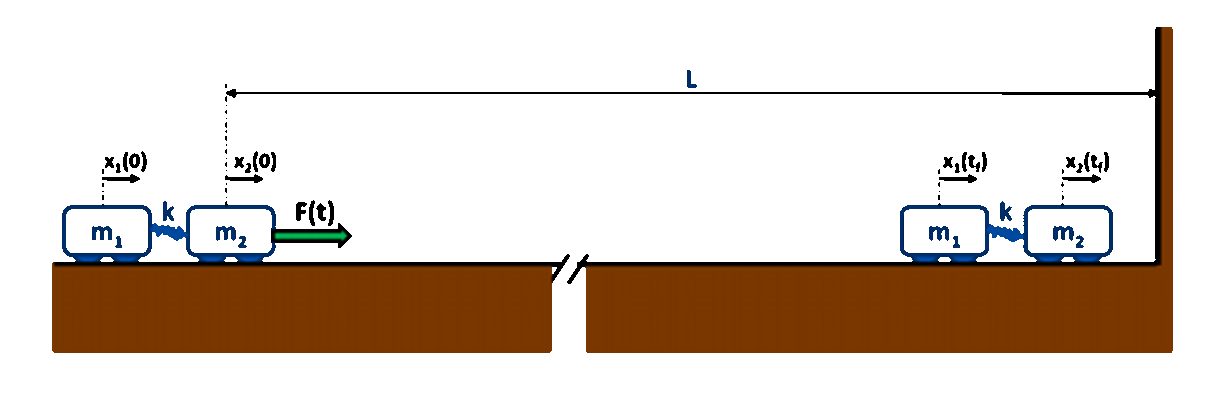
\includegraphics[width=0.8\textwidth]{media/image7}\\
    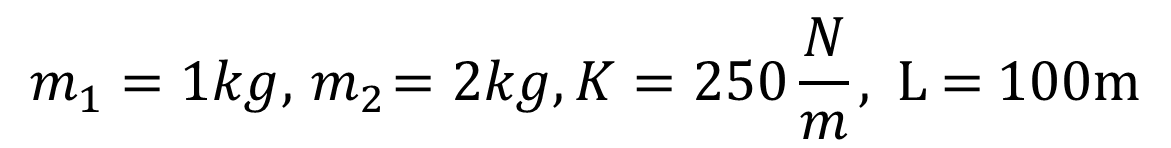
\includegraphics[width=0.8\textwidth]{media/image8}
\end{frame}

\begin{frame}{Problem Statement (2/3)}
    \centering
    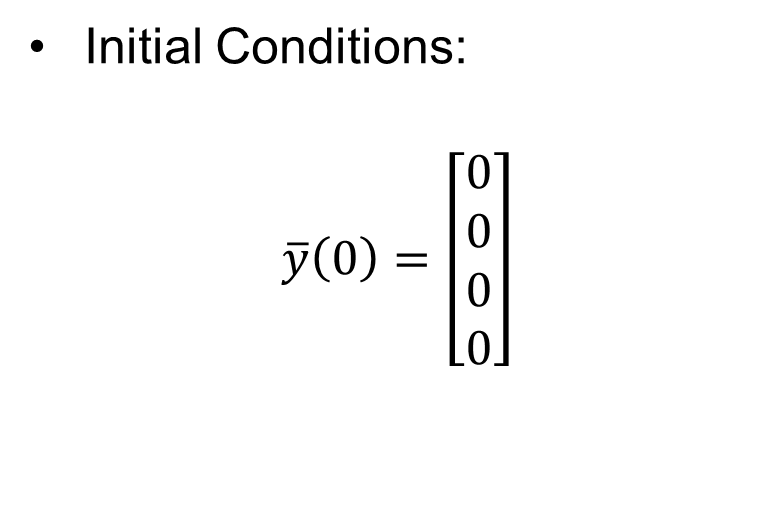
\includegraphics[width=0.4\textwidth]{media/image9}
    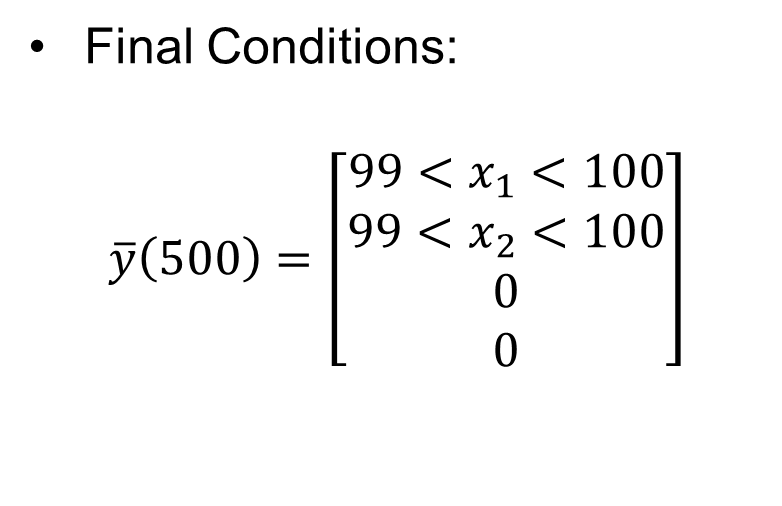
\includegraphics[width=0.4\textwidth]{media/image10}\\
    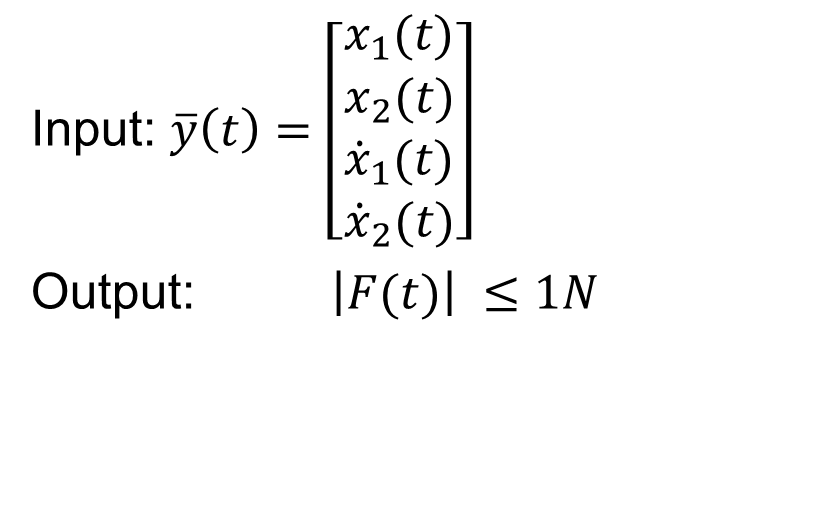
\includegraphics[width=0.4\textwidth]{media/image11}
\end{frame}

\begin{frame}{Problem Statement (3/3)}
    \centering
    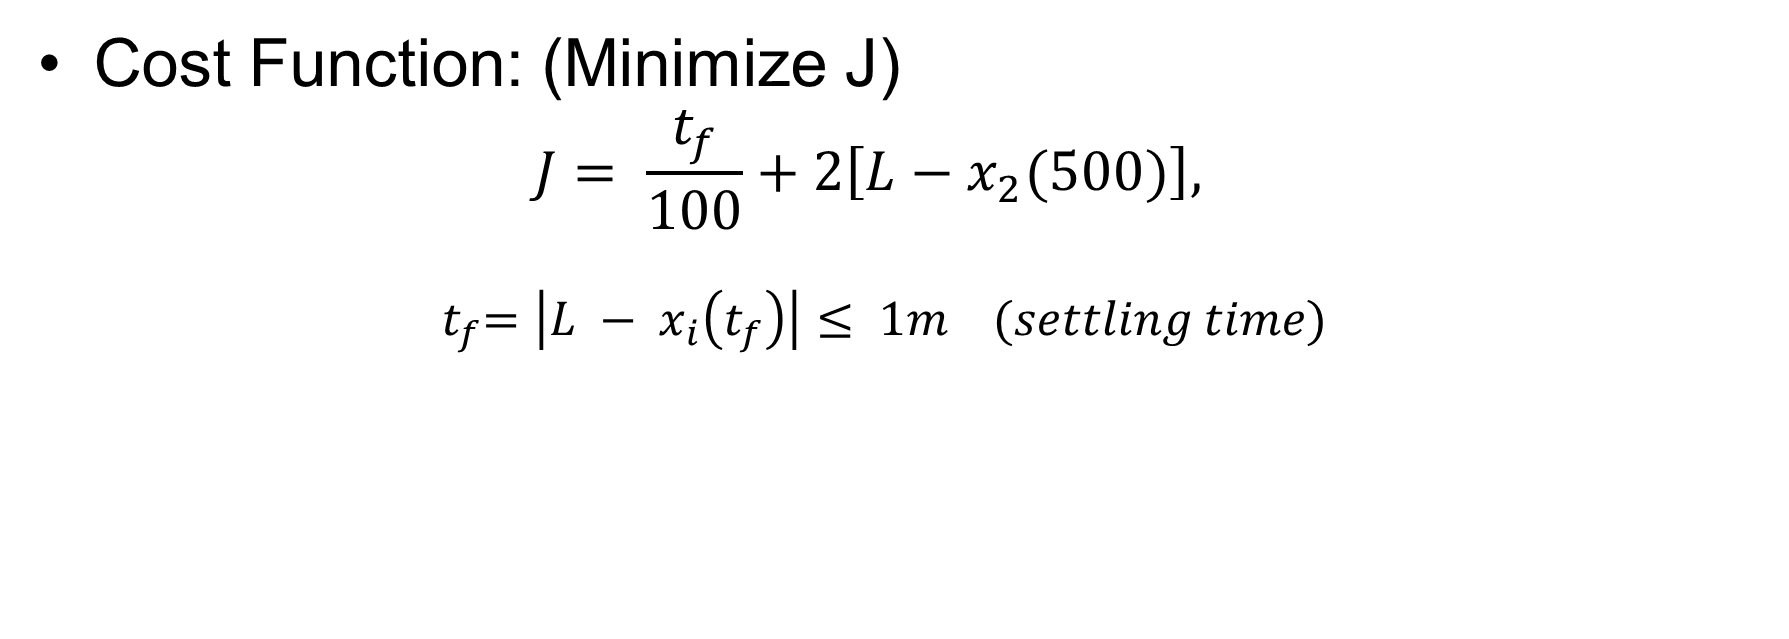
\includegraphics[width=0.8\textwidth]{media/image13}\\
    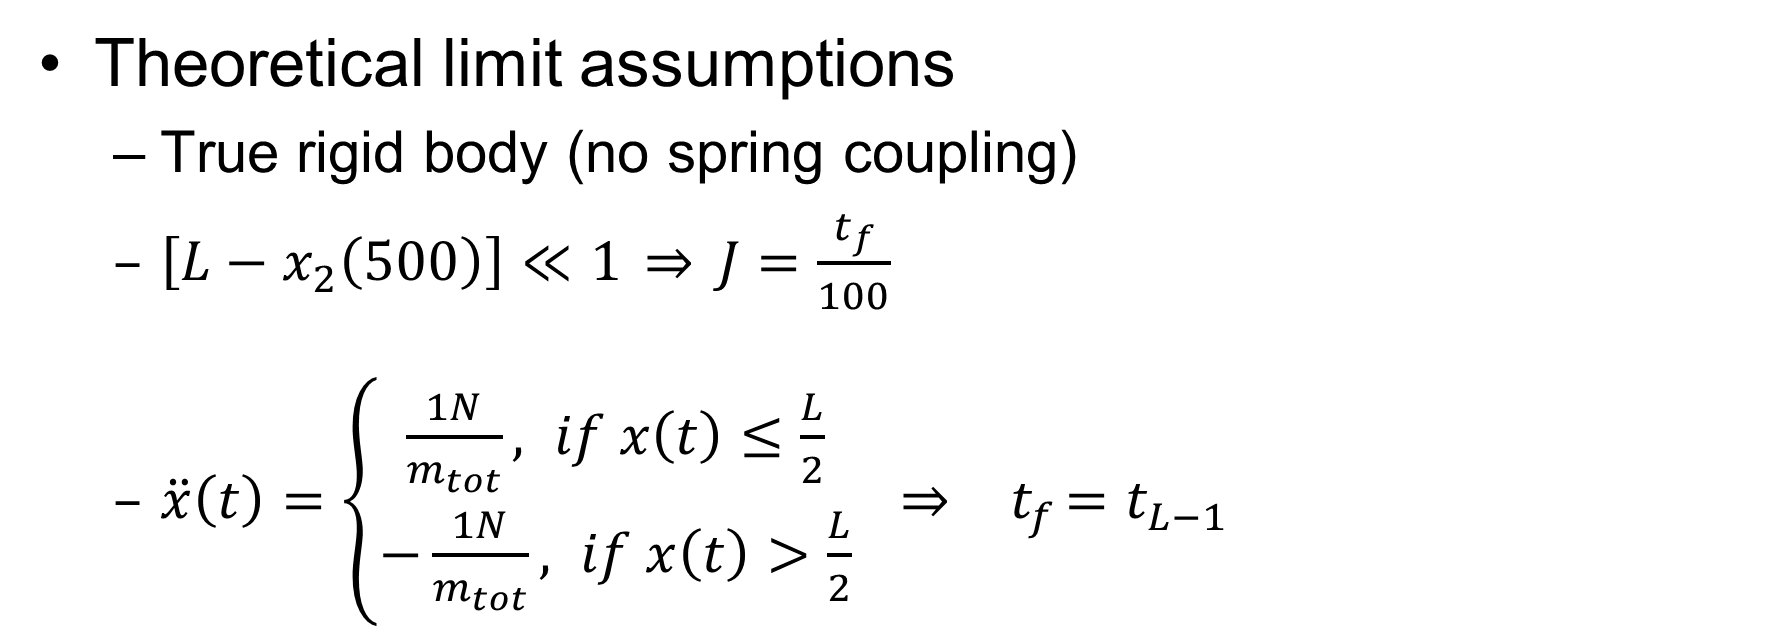
\includegraphics[width=0.8\textwidth]{media/image14}
\end{frame}

\begin{frame}{Inputs}
    \begin{columns}
        \begin{column}{0.5\textwidth}
            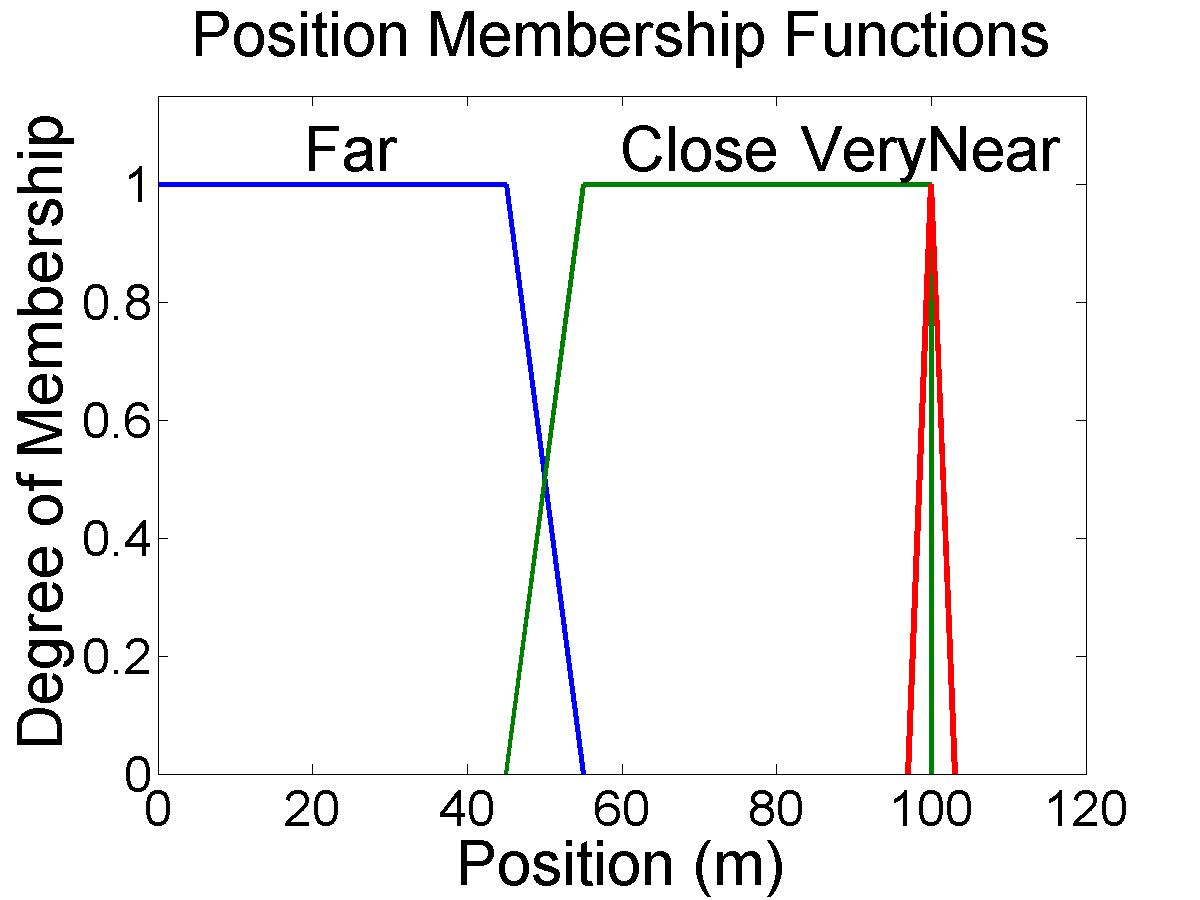
\includegraphics[width=\textwidth]{media/image17}
        \end{column}
        \begin{column}{0.5\textwidth}
            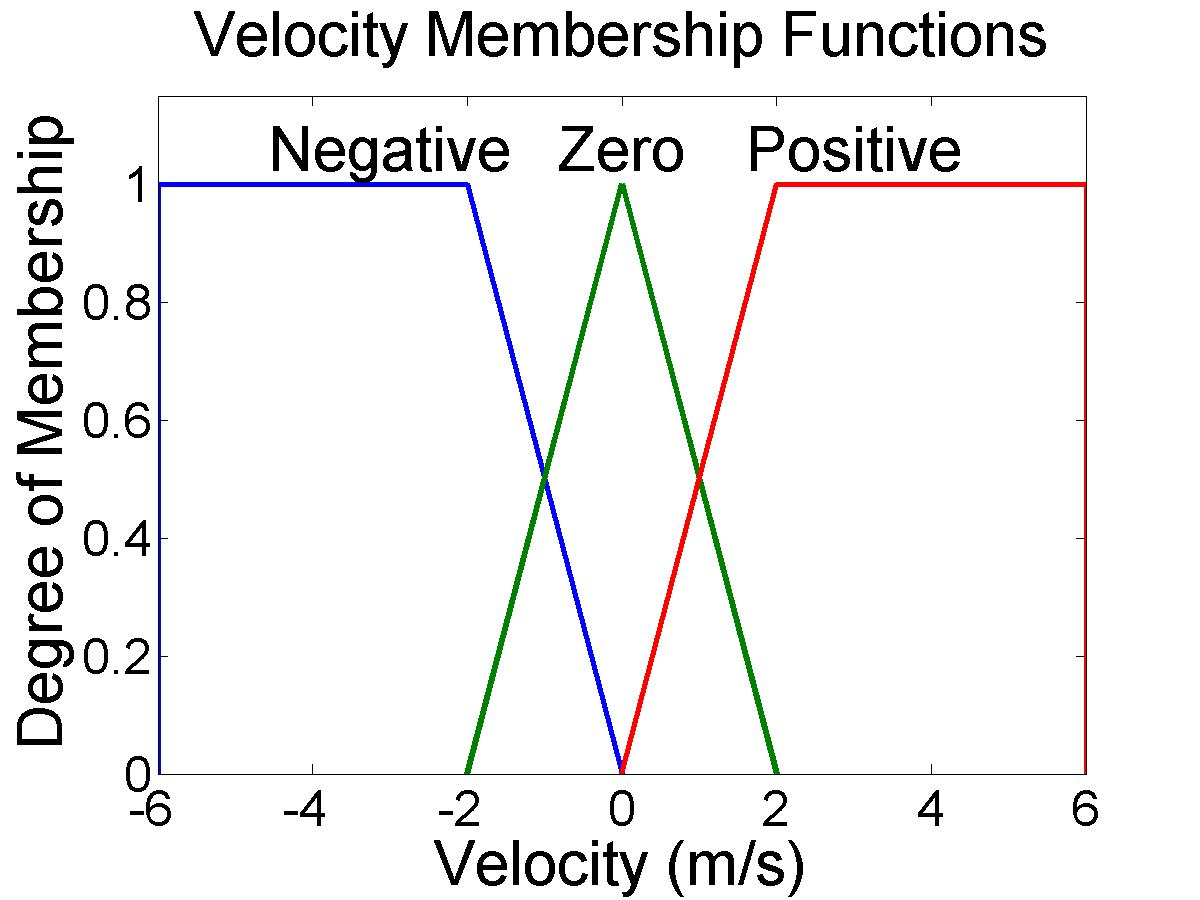
\includegraphics[width=\textwidth]{media/image18}
        \end{column}
    \end{columns}
\end{frame}

\begin{frame}{Output}
    \centering
    \vspace{2em}
    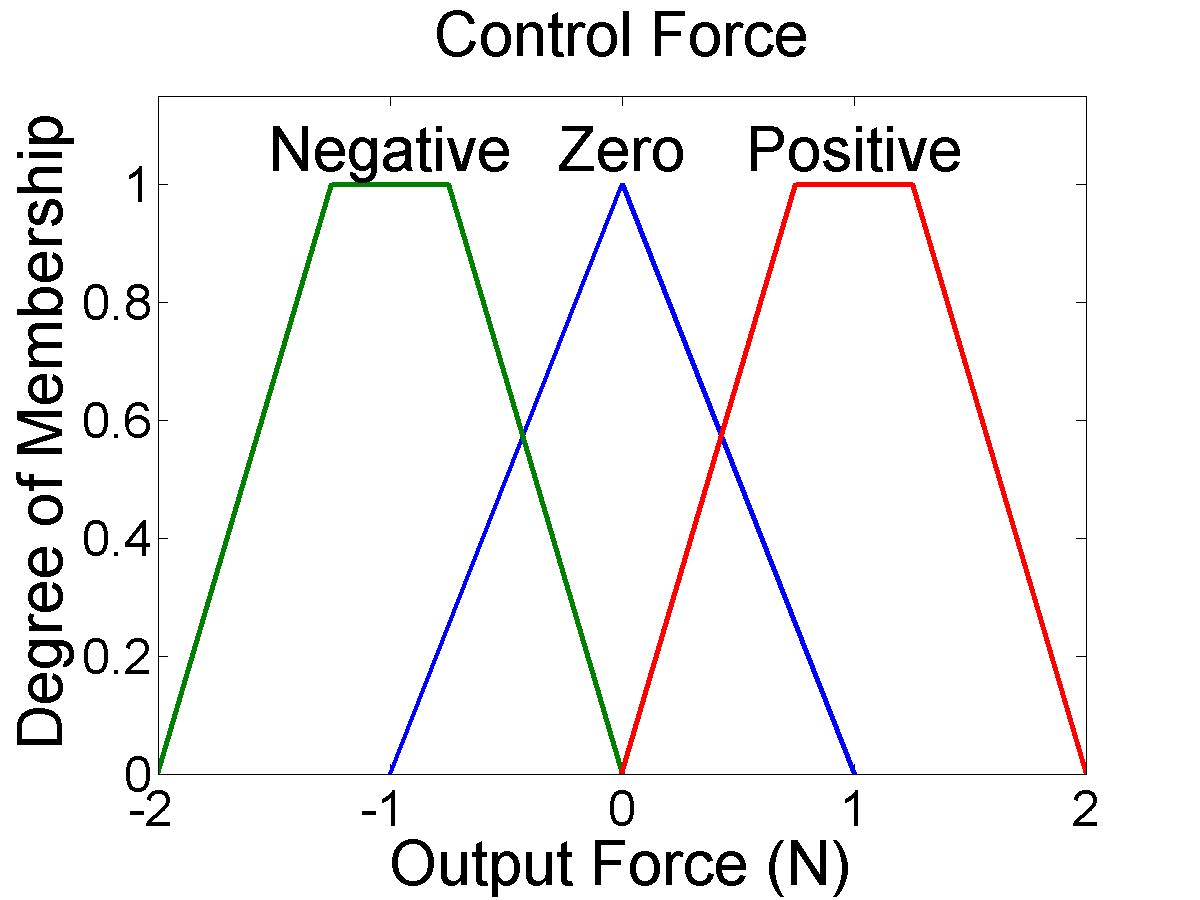
\includegraphics[width=0.8\textwidth]{media/image19}
\end{frame}

\begin{frame}{Rule Base}
    \centering
    \vspace{2em}
    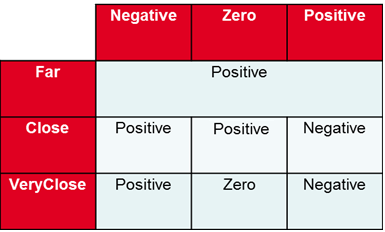
\includegraphics[width=0.7\textwidth]{media/image20}
\end{frame}

\begin{frame}{Search Space Reduction}
            \centering
            \vspace{2em}
            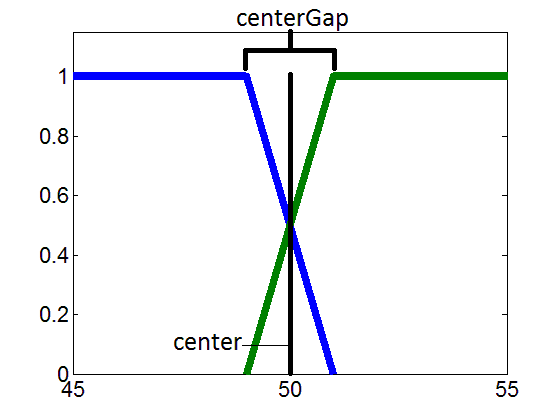
\includegraphics[width=0.4\textwidth]{media/image21}
            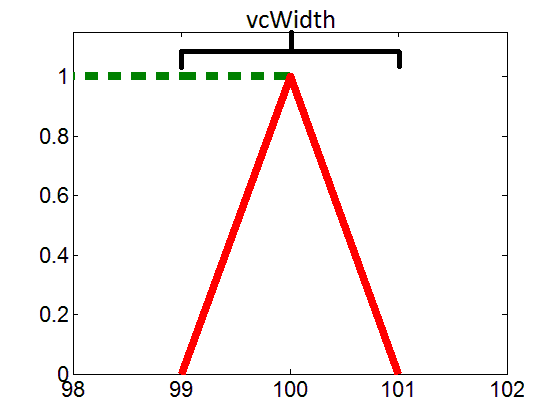
\includegraphics[width=0.4\textwidth]{media/image22}\\
            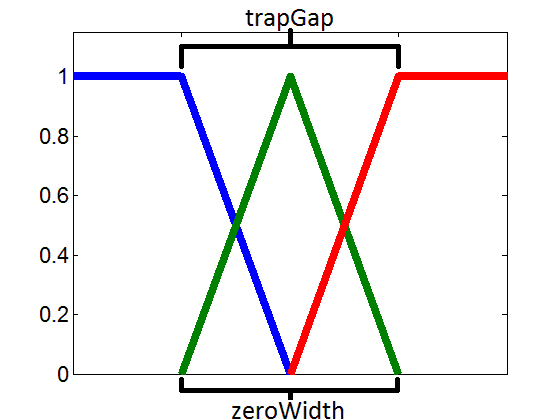
\includegraphics[width=0.4\textwidth]{media/image23}
            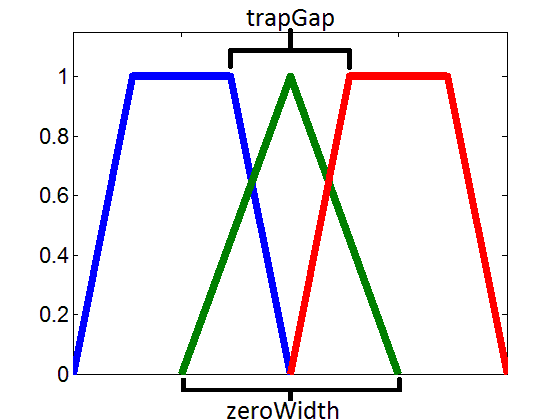
\includegraphics[width=0.4\textwidth]{media/image24}
\end{frame}

\begin{frame}{Results}
    \centering
    \vspace{2em}
    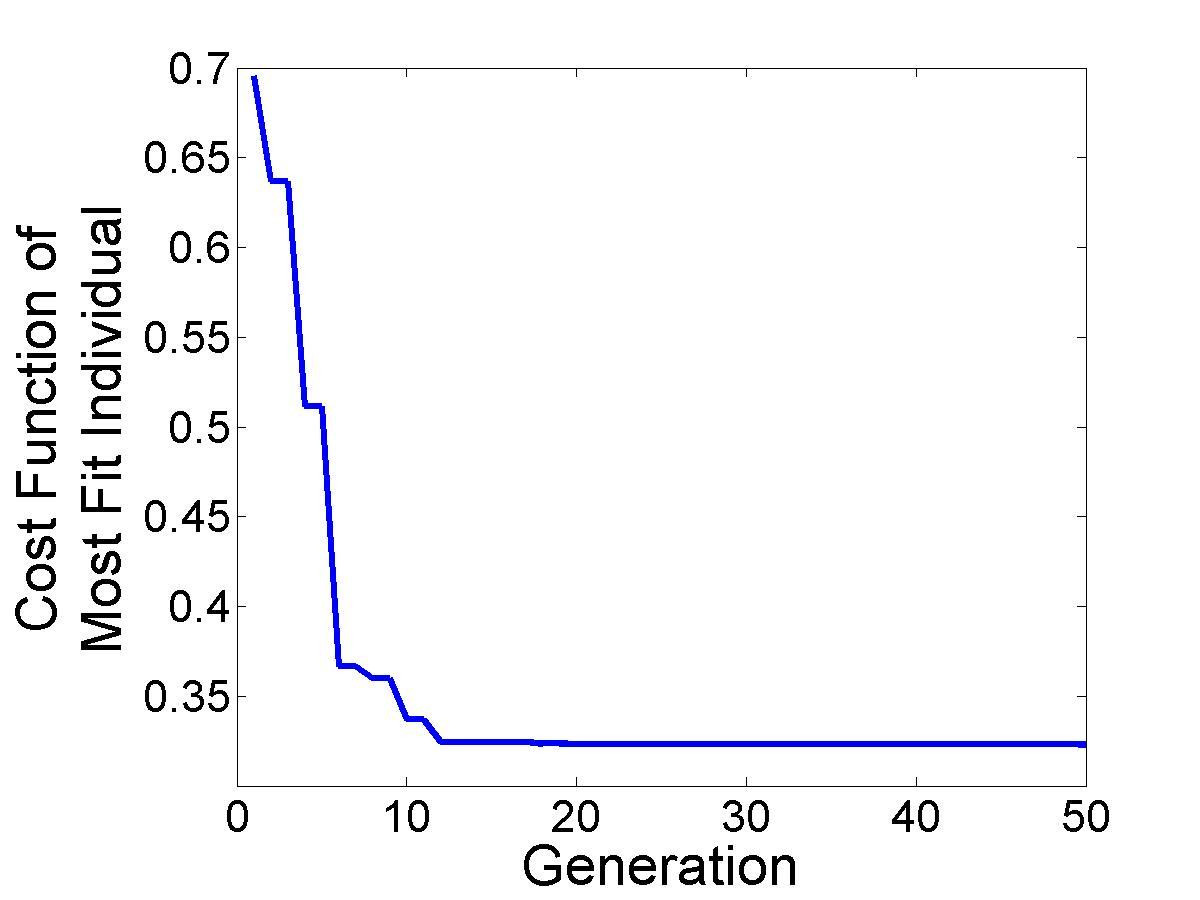
\includegraphics[width=0.6\textwidth]{media/image38}\\
    \begin{tabular}{|c|c|c|} \hline
        $t_f$ & $x_2(500)$ & $J$ \\\hline
        \SI{32.308}{\second} & \SI{99.999999}{\metre} &  0.32311 \\\hline
    \end{tabular} 
\end{frame}

\begin{frame}{Robustness Results}
    \begin{tabular}{|c|c|c|c|c|} \cline{2-5}
        \multicolumn{1}{c|}{} & \multicolumn{4}{|c|}{Mass 1 (\si{\kilogram}), Mass 2 (\si{\kilogram})} \\\cline{2-5}
        \multicolumn{1}{c|}{} & \SI{1}{\kilogram}, \SI{2}{\kilogram} & \SI{2}{\kilogram}, \SI{4}{\kilogram} & \SI{4}{\kilogram}, \SI{8}{\kilogram} & \SI{4}{\kilogram}, \SI{16}{\kilogram} \\\hline
        Theoretical Limit & 0.3191 & 0.4553 & 0.6438 & 0.8312 \\\hline
        GA FIS & 0.3231 & 0.4562 & 0.6579 & 0.8434 \\\hline
        Hand-tuned FIS & 0.3233 & 0.6125 & 5.3072 & 3.3240 \\\hline\hline
        GA Error & \multicolumn{1}{|d|}{1.3\%} & \multicolumn{1}{|d|}{0.2\%} & \multicolumn{1}{|d|}{2.2\%} & \multicolumn{1}{|d|}{1.5\%} \\\hline
        Hand-tuned Error & \multicolumn{1}{|d|}{1.3\%} & \multicolumn{1}{|d|}{34.5\%} & \multicolumn{1}{|d|}{724.4\%} & \multicolumn{1}{|d|}{299.9\%} \\\hline 
    \end{tabular}
\end{frame}

\section{F-4 Pitch Attitude Control System}
\begin{frame}{The Problem}
\begin{itemize}
\item F4 Attitude Pitch Attitude Hold System
    \begin{itemize}
    \item Chosen for interesting/challenging dynamics
        \begin{itemize}
        \item Has zeros located close to origin
        \item Poles close to imaginary axis
        \end{itemize}
    \item 4 Cases tested
        \begin{itemize}
        \item Nominal approach
        \item 50\% degradation in aerodynamic derivatives
        \item Nominal subsonic cruise
        \item Nominal supersonic cruise
        \end{itemize}
    \item Covers large portion of F4 flight envelope
    \end{itemize}
\end{itemize}
\end{frame}


\begin{frame}{The Problem}
\begin{itemize}
\item Traditional PID design
    \begin{itemize}
    \item The good
        \begin{itemize}
        \item Well understood
        \item Relatively easy to tune
        \item Computationally simple
        \end{itemize}
    \item The bad
        \begin{itemize}
        \item Inflexible to changes in plant
        \item Unintelligent, non-adaptive control
        \item Change in plant may lead to unstable control behavior
        \end{itemize}
    \end{itemize}
\end{itemize}
\end{frame}
\note{Gain scheduling can help here, but is also problematic}

\begin{frame}{The Solution (part I)}
\begin{itemize}
\item Fuzzy PID
    \begin{itemize}
    \item The good
        \begin{itemize}
        \item Adaptive
        \item Continuous, intuitive gain scheduling
        \item Allows gains to `float' around to best fit the situation
        \item Best of both worlds
        \end{itemize}
    \item The bad
        \begin{itemize}
        \item Hard to tune
        \end{itemize}
    \end{itemize}
\end{itemize}
\end{frame}


\begin{frame}{The Solution (part II)}
\begin{itemize}
\item Genetic Fuzzy
    \begin{itemize}
    \item The good
        \begin{itemize}
        \item\only<1>{Self-tuning}
        \only<2->{\st{Self-tuning} Self-learning}
        \item<3-> Removes the iterative tedium from the control engineer\only<4->{ (mostly)}
        \end{itemize}
    \item<4-> The bad
        \begin{itemize}
        \item<5-> Non-deterministic optimization algorithm
        \item<6-> Resistant to validation and verification
        \item<7-> Highly dependent on cost function
        \item<8-> Needs TIME/DATA
        \end{itemize}
    \end{itemize}
\end{itemize}
\end{frame}

\begin{frame}{Generic Parameters}
    \begin{itemize}
        \item Genetic Algorithm
            \begin{itemize}
                \item Population Size: 100
                \item Maximum Generation: 200
            \end{itemize}
        \item Fuzzy Inference System
            \begin{itemize}
                \item 3 input ($e,\;\sum e,\;\Delta e$), 3 output ($k_p,\;k_i,\;k_d$)
                \item Membership functions per fuzzy partition: 5
                \item Number of fuzzy rules: 125
            \end{itemize}
        \item Cost Function
            \begin{itemize}
                \item $ J = T_s$
            \end{itemize}
    \end{itemize}
\end{frame}

\begin{frame}{Nominal Condition}
    \begin{columns}
        \begin{column}{0.5\textwidth}
            \vspace{-3.25cm}
            \begin{itemize}
                \item Fuzzy PID Response
                    \begin{tabular}{cccccc}
                        &$T_s$ & $T_r$ & $T_p$ & $M_p$ & FV\\\cline{2-6}
                        & 1.86 & 0.26 & 0.66 & 1.396 & 1.00\\\hline

                    \end{tabular}
                \item PID Response
                    \begin{tabular}{cccccc}
                        &$T_s$ & $T_r$ & $T_p$ & $M_p$ & FV\\\cline{2-6}
                        & 7.08      & 1.27      & 4.98      & 1.023       & 1.00 
                    \end{tabular}
            \end{itemize}
        \end{column}
        \begin{column}{0.5\textwidth}
            \centering
            \vspace{3.25cm}
            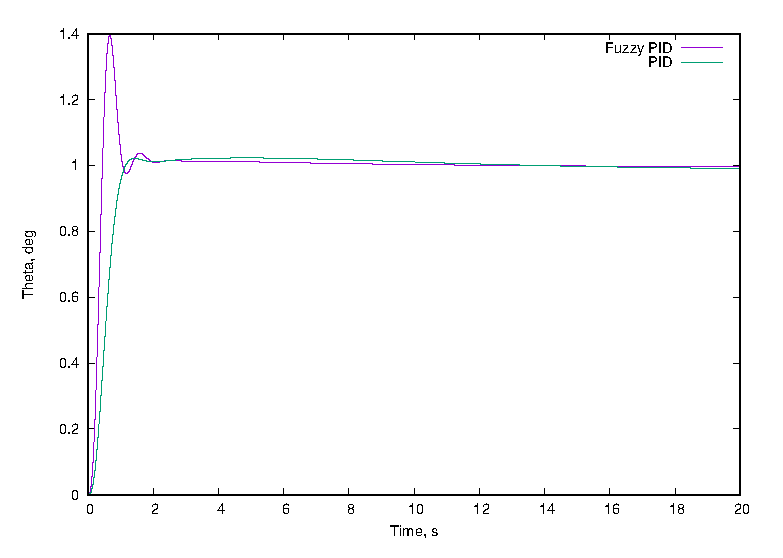
\includegraphics[width=\textwidth]{\resdir/f4_approach}
        \end{column}
    \end{columns}
\end{frame}

\begin{frame}{Degraded Condition}
    \begin{columns}
        \begin{column}{0.5\textwidth}
            \vspace{-3.25cm}
            \begin{itemize}
                \item Fuzzy PID Response
                    \begin{tabular}{cccccc}
                        &$T_s$ & $T_r$ & $T_p$ & $M_p$ & FV\\\cline{2-6}
                        & 4.09 & 0.28 & 0.68 & 1.239 & 1.00\\\hline

                    \end{tabular}
                \item PID Response
                    \begin{tabular}{cccccc}
                        &$T_s$ & $T_r$ & $T_p$ & $M_p$ & FV\\\cline{2-6}
                        & 1.66      & 1.69      & 1.75      & 1.014       & 1.00
                    \end{tabular}
            \end{itemize}
        \end{column}
        \begin{column}{0.5\textwidth}
            \centering
            \vspace{3.25cm}
            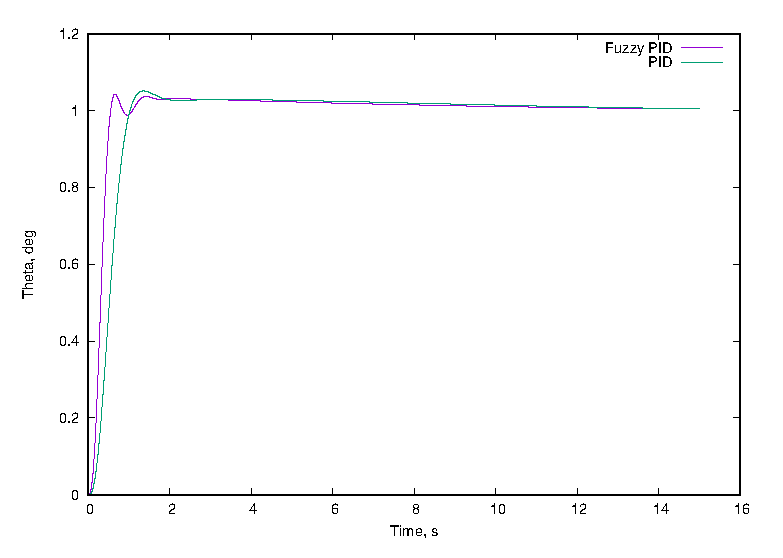
\includegraphics[width=\textwidth]{\resdir/f4_deg}
        \end{column}
    \end{columns}
\end{frame}

\begin{frame}{Adjusted Cost Function}
            \begin{itemize}
                \item $J = T_s + 3\cdot OS\%$
                \item Fuzzy PID Response
                    \begin{tabular}{cccccc}
                        &$T_s$ & $T_r$ & $T_p$ & $M_p$ & FV\\\cline{2-6}
                        & 1.86 & 0.26 & 0.66 & 1.396 & 1.00\\\hline

                    \end{tabular}
                \item PID Response
                    \begin{tabular}{cccccc}
                        &$T_s$ & $T_r$ & $T_p$ & $M_p$ & FV\\\cline{2-6}
                        & 4.09 & 0.28 & 0.68 & 1.239 & 1.00\\\hline

                    \end{tabular}
            \end{itemize}
\end{frame}

\begin{frame}{Nominal Condition - Modified Cost Function}
    \centering
    \vspace{1cm}
    \includegraphics[width=0.8\textwidth]{\resdir/test/f4_approach-eps-converted-to}
\end{frame}

\begin{frame}{Degraded Condition - Modified Cost Function}
    \centering
    \vspace{1cm}
    \includegraphics[width=0.8\textwidth]{\resdir/test/f4_deg-eps-converted-to}
\end{frame}

\section{Precision Landing System}
\begin{frame}{Background}
    \begin{itemize}
        \item Develop control strategy for robust, precision landing
            \begin{itemize}
                \item Place focus on implementable control
                \item Approach from hardware constraints
                \item Controller must be onboard
            \end{itemize}
        \item Use vision-based sensors only for guidance
            \begin{itemize}
                \item Ubiquitous
                \item Cheap
                \item No special sensors required
            \end{itemize}
        \item Target available hardware in the lab
        \item Caveats
            \begin{itemize}
                \item Target platform motion constrained to level plane
            \end{itemize}
    \end{itemize}
\end{frame}

\begin{frame}{Flight Hardware}
    \centering
    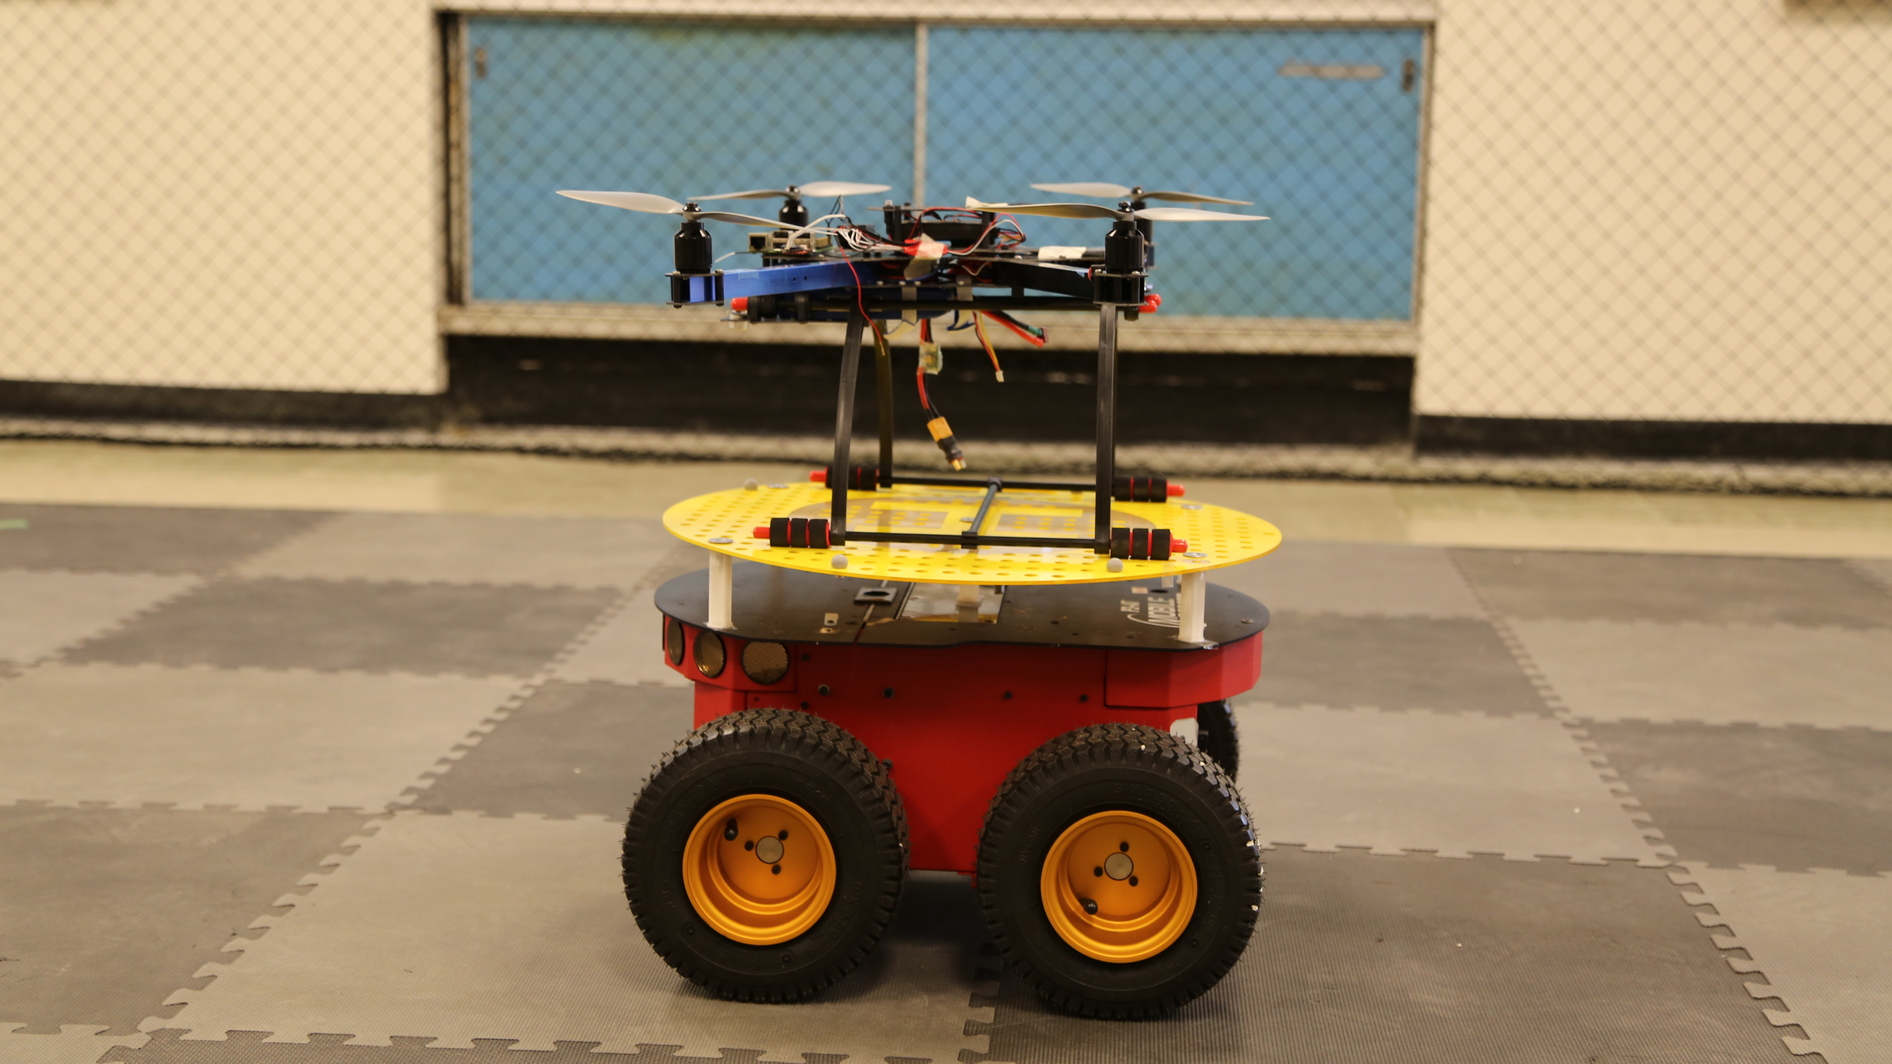
\includegraphics[width=0.8\textwidth]{../images/irols.png}
\end{frame}

\begin{frame}{Control Architecture}
    \begin{columns}
        \begin{column}{0.45\textwidth}
            \begin{itemize}
                \item State vector
                    \begin{itemize}
                        \item $\bm{x} = \left[x,y,z,\psi\right]^\top$
                    \end{itemize}
                \item Control
                    \begin{itemize}
                        \item Input: $\Delta\bm{x},\,\dot{\Delta\bm{x}}$
                        \item Output: $\bm{u}=\left[\dot{x},\dot{y},\dot{z},\dot{\psi}\right]^\top$
                    \end{itemize}
                \item Fuzzy Logic Controller (FLC)
                    \begin{itemize}
                        \item Computationally inexpensive
                        \item Tolerant of noisy data
                    \end{itemize}
            \end{itemize}
        \end{column}
        \begin{column}{0.55\textwidth}
            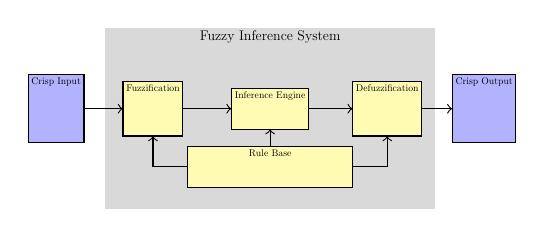
\begin{tikzpicture}[scale=0.35, transform shape]
    \node[fill=gray!30,text depth = 6cm,minimum width=12cm,font=\Large] (main){Fuzzy Inference System};
    \node[draw,fill=yellow!30, text depth=1cm] at ([yshift=1em]main.center)(infer){Inference Engine};
    \node[draw,fill=yellow!30, text depth=1cm, minimum width=6cm] at ([yshift=-5em]main.center)(rb){Rule Base};
    \node[draw,fill=yellow!30, text depth=1.5cm] at ([xshift=5em, yshift=1em]main.west)(fuzz){Fuzzification};
    \node[draw,fill=yellow!30, text depth=1.5cm] at ([xshift=-5em, yshift=1em]main.east)(defuzz){Defuzzification};
    \node[draw,fill=blue!30, text depth=2cm] at ([xshift=-5em, yshift=1em]main.west)(inp){Crisp Input};
    \node[draw,fill=blue!30, text depth=2cm] at ([xshift=5em, yshift=1em]main.east)(outp){Crisp Output};

    \node at ([xshift=5em, yshift=-5em]main.west)(ghostleft){};
    \node at ([xshift=-5em, yshift=-5em]main.east)(ghostright){};

    \draw[->](inp.east) -- (fuzz.west);
    \draw[->](fuzz.east) -- (infer.west);
    \draw[->](infer.east) -- (defuzz.west);
    \draw[->](defuzz.east) -- (outp.west);
    \draw[->](rb.north) -- (infer.south);
    \draw[->](rb.west) -- (ghostleft.center) -- (fuzz.south);
    \draw[->](rb.east) -- (ghostright.center) -- (defuzz.south);
\end{tikzpicture}

        \end{column}
    \end{columns}
\end{frame}
            

\begin{frame}{Approach}
    \begin{columns}
        \begin{column}{0.4\textwidth}
            \begin{itemize}
                \item Simulate
                    \begin{itemize}
                        \item Gazebo
                        \item Full-featured simulation
                        \item Full hardware emulation
                    \end{itemize}
                \item Tune/Iterate
                    \begin{itemize}
                        \item Evolutionary learning
                    \end{itemize}
                \item Build
                    \begin{itemize}
                        \item Hardware implementation
                    \end{itemize}
            \end{itemize}
        \end{column}
        \begin{column}{0.55\textwidth}
            \includegraphics[width=1.0\textwidth]{../images/gazebosim_landing}
        \end{column}
    \end{columns}
\end{frame}


\begin{frame}{Tools}
    \begin{itemize}
        \item Robot Operating System
            \begin{itemize}
                \item Distributed execution framework
                \item Message marshalling
                \item Publish/Subscribe model
            \end{itemize}
        \item Gazebo
            \begin{itemize}
                \item 3D dynamics simulator
                \item Sensor simulation
            \end{itemize}
        \item AprilTags
            \begin{itemize}
                \item Visual fiducial system for robotics
                \item Developed by Univ. of Michigan
                \item Robust and lightweight (small data payloads)
            \end{itemize}
    \end{itemize}
\end{frame}

\begin{frame}{ROS (1/2)}
    \centering
    \includedot[scale=0.135]{../tikz/rosgraph}
    \vspace{2em}
    ROS handles a lot of complexity for the end user. Allows building complex, scalable systems.
\end{frame}

\begin{frame}{ROS (2/2)}
    \begin{columns}
        \begin{column}{0.3\textwidth}
            \begin{itemize}
                \item SMACH (State MACHine)
                    \begin{itemize}
                        \item Decompose problem into states
                        \item Chain states with transitions
                        \item Allows to focus on micro behavior
                    \end{itemize}
            \end{itemize}
        \end{column}
        \begin{column}{0.7\textwidth}
            \includedot[scale=0.2]{../tikz/smach}
        \end{column}
    \end{columns}
\end{frame}

\begin{frame}{Homography}
    \begin{itemize}
        \item Altitude estimation
            \begin{itemize}
                \item Use GPS/Baraometer until target is visible
                \item Estimate altitude from known size of target
                    \begin{itemize}
                        \item Circular Area (px) $\rightarrow$ Diameter (px) $\rightarrow$ $\frac{d\cdot
                            f}{m\cdot d_p}\rightarrow d_z$
                    \end{itemize}
                \item Use AprilTag detection if available
                    \begin{itemize}
                        \item Needed for target occlusion, frame saturation
                    \end{itemize}
            \end{itemize}
        \item Position (2D) estimation
            \begin{itemize}
                \item Relative to target position
                \item EKF fusion of visual track, AprilTag track, and IMU information
            \end{itemize}
    \end{itemize}
\end{frame}

\begin{frame}{Homography}
    \setbeamercolor{normal text}{fg=gray!30,bg=}
    \setbeamercolor{alerted text}{fg=black,bg=}
    \usebeamercolor{normal text}
    \begin{itemize}
        \item \alert{Visual estimate is obtained by mapping the projected target image onto world coordinates}
        \item \alert<+>{
            \begin{math}
                \bm{R}(\phi,\theta,\psi) = 
                \begin{bmatrix}
                    c_{\theta}c_{\psi}                           & -c_{\theta}s_{\phi}                           & s_{\theta}\\
                    c_{\phi}s_{\psi} + c_{\psi}s_{\phi}s_{\theta} & c_{\phi}c_{\psi} - c_{\psi}s_{\phi}s_{\theta} & -c_{\theta}s_{\phi}\\
                    s_{\phi}s_{\psi} -c_{\phi}c_{\psi}s_{\theta} & c_{\psi}s_{\phi} + c_{\phi}s_{\theta}s_{\psi} & c_{\phi}c_{\theta}
                \end{bmatrix}
            \end{math} }
        \item \alert<+>{
            \begin{math}
                \bm{R}_{cam}^{body}    = R(\pi, 0, 0)\quad
                \bm{R}_{body}^{inert}  = R(\phi, \theta, \psi)
            \end{math} }
        \item \alert<+>{Projected position of target center parallel to image plane:\\
            \begin{math}
            p_i = \begin{pmatrix}d_x\\d_y\\d_z\end{pmatrix}
            \end{math} }
        \item \alert<+>{Relative position of target in inertial frame:\\
            \begin{math}
                p_r = \bm{R}_{body}^{inert}\bm{R}_{cam}^{body}p_i
            \end{math} }
    \end{itemize}
\end{frame}

\begin{frame}{Pose Estimation}
    %\begin{subfigmatrix}{4}% number of columns
    \centering
        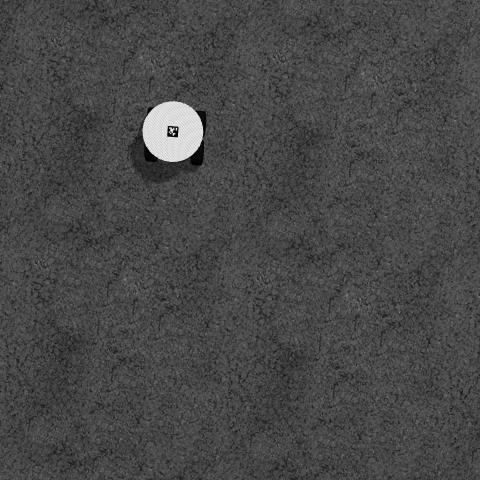
\includegraphics[width=0.2\textwidth]{../images/image2_18469000.png}
        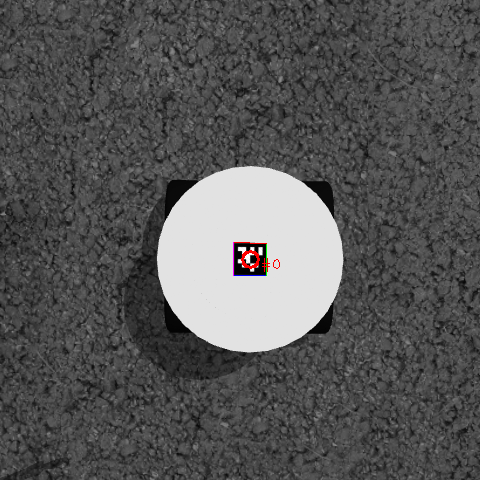
\includegraphics[width=0.2\textwidth]{../images/image2_30863000.png}
        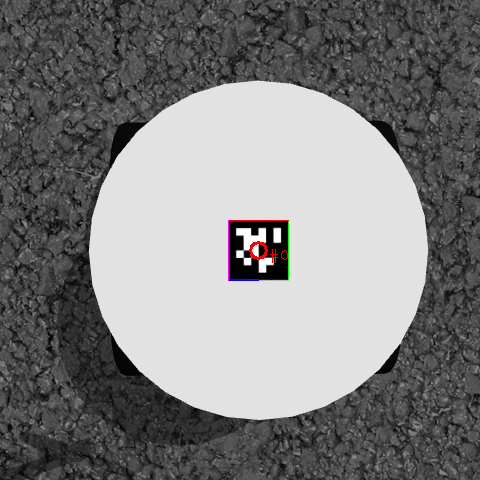
\includegraphics[width=0.2\textwidth]{../images/image2_36074000.png}
        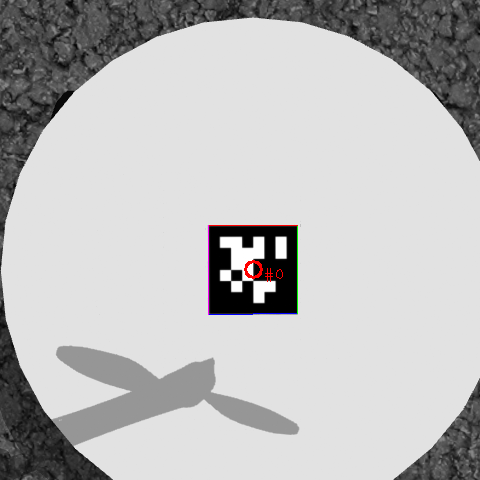
\includegraphics[width=0.2\textwidth]{../images/image2_38233000.png}\\
        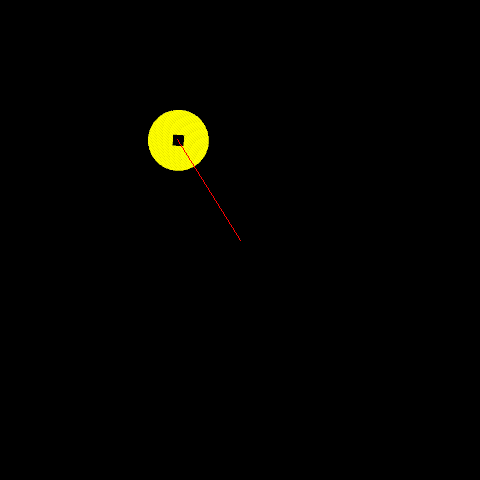
\includegraphics[width=0.2\textwidth]{../images/image1_18469000_proc.png}
        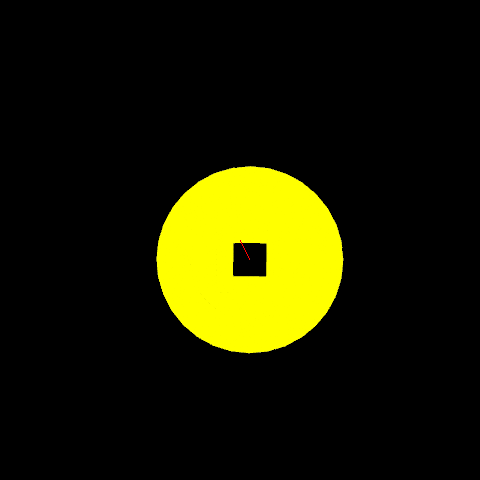
\includegraphics[width=0.2\textwidth]{../images/image1_30863000_proc.png}
        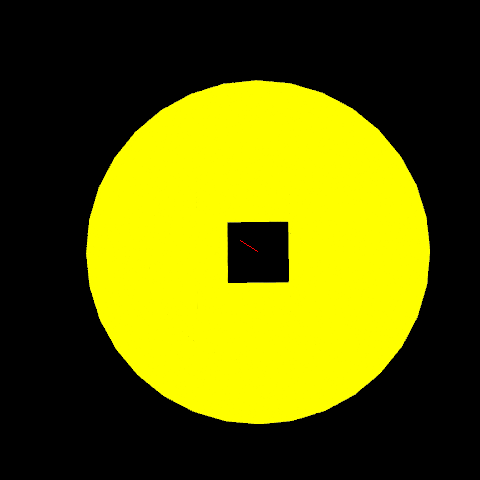
\includegraphics[width=0.2\textwidth]{../images/image1_36074000_proc.png}
        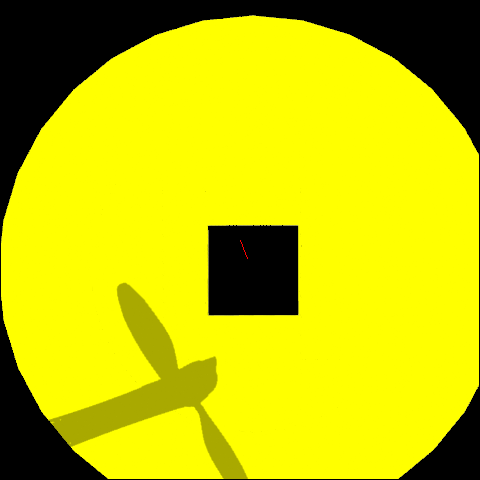
\includegraphics[width=0.2\textwidth]{../images/image1_38233000_proc.png}
    %\end{subfigmatrix}
\end{frame}

{
    \usebackgroundtemplate{}
\begin{frame}[fragile]{Extended Kalman Filter}
    \begin{overlayarea}{\textwidth}{6cm}
        \onslide<1>
        \scalebox{0.8}{% GNUPLOT: LaTeX picture with Postscript
\begingroup
  \makeatletter
  \providecommand\color[2][]{%
    \GenericError{(gnuplot) \space\space\space\@spaces}{%
      Package color not loaded in conjunction with
      terminal option `colourtext'%
    }{See the gnuplot documentation for explanation.%
    }{Either use 'blacktext' in gnuplot or load the package
      color.sty in LaTeX.}%
    \renewcommand\color[2][]{}%
  }%
  \providecommand\includegraphics[2][]{%
    \GenericError{(gnuplot) \space\space\space\@spaces}{%
      Package graphicx or graphics not loaded%
    }{See the gnuplot documentation for explanation.%
    }{The gnuplot epslatex terminal needs graphicx.sty or graphics.sty.}%
    \renewcommand\includegraphics[2][]{}%
  }%
  \providecommand\rotatebox[2]{#2}%
  \@ifundefined{ifGPcolor}{%
    \newif\ifGPcolor
    \GPcolortrue
  }{}%
  \@ifundefined{ifGPblacktext}{%
    \newif\ifGPblacktext
    \GPblacktexttrue
  }{}%
  % define a \g@addto@macro without @ in the name:
  \let\gplgaddtomacro\g@addto@macro
  % define empty templates for all commands taking text:
  \gdef\gplbacktext{}%
  \gdef\gplfronttext{}%
  \makeatother
  \ifGPblacktext
    % no textcolor at all
    \def\colorrgb#1{}%
    \def\colorgray#1{}%
  \else
    % gray or color?
    \ifGPcolor
      \def\colorrgb#1{\color[rgb]{#1}}%
      \def\colorgray#1{\color[gray]{#1}}%
      \expandafter\def\csname LTw\endcsname{\color{white}}%
      \expandafter\def\csname LTb\endcsname{\color{black}}%
      \expandafter\def\csname LTa\endcsname{\color{black}}%
      \expandafter\def\csname LT0\endcsname{\color[rgb]{1,0,0}}%
      \expandafter\def\csname LT1\endcsname{\color[rgb]{0,1,0}}%
      \expandafter\def\csname LT2\endcsname{\color[rgb]{0,0,1}}%
      \expandafter\def\csname LT3\endcsname{\color[rgb]{1,0,1}}%
      \expandafter\def\csname LT4\endcsname{\color[rgb]{0,1,1}}%
      \expandafter\def\csname LT5\endcsname{\color[rgb]{1,1,0}}%
      \expandafter\def\csname LT6\endcsname{\color[rgb]{0,0,0}}%
      \expandafter\def\csname LT7\endcsname{\color[rgb]{1,0.3,0}}%
      \expandafter\def\csname LT8\endcsname{\color[rgb]{0.5,0.5,0.5}}%
    \else
      % gray
      \def\colorrgb#1{\color{black}}%
      \def\colorgray#1{\color[gray]{#1}}%
      \expandafter\def\csname LTw\endcsname{\color{white}}%
      \expandafter\def\csname LTb\endcsname{\color{black}}%
      \expandafter\def\csname LTa\endcsname{\color{black}}%
      \expandafter\def\csname LT0\endcsname{\color{black}}%
      \expandafter\def\csname LT1\endcsname{\color{black}}%
      \expandafter\def\csname LT2\endcsname{\color{black}}%
      \expandafter\def\csname LT3\endcsname{\color{black}}%
      \expandafter\def\csname LT4\endcsname{\color{black}}%
      \expandafter\def\csname LT5\endcsname{\color{black}}%
      \expandafter\def\csname LT6\endcsname{\color{black}}%
      \expandafter\def\csname LT7\endcsname{\color{black}}%
      \expandafter\def\csname LT8\endcsname{\color{black}}%
    \fi
  \fi
    \setlength{\unitlength}{0.0500bp}%
    \ifx\gptboxheight\undefined%
      \newlength{\gptboxheight}%
      \newlength{\gptboxwidth}%
      \newsavebox{\gptboxtext}%
    \fi%
    \setlength{\fboxrule}{0.5pt}%
    \setlength{\fboxsep}{1pt}%
\begin{picture}(7200.00,5040.00)%
    \gplgaddtomacro\gplbacktext{%
      \csname LTb\endcsname%
      \put(946,704){\makebox(0,0)[r]{\strut{}$0$}}%
      \put(946,1156){\makebox(0,0)[r]{\strut{}$0.01$}}%
      \put(946,1609){\makebox(0,0)[r]{\strut{}$0.02$}}%
      \put(946,2061){\makebox(0,0)[r]{\strut{}$0.03$}}%
      \put(946,2513){\makebox(0,0)[r]{\strut{}$0.04$}}%
      \put(946,2966){\makebox(0,0)[r]{\strut{}$0.05$}}%
      \put(946,3418){\makebox(0,0)[r]{\strut{}$0.06$}}%
      \put(946,3870){\makebox(0,0)[r]{\strut{}$0.07$}}%
      \put(946,4323){\makebox(0,0)[r]{\strut{}$0.08$}}%
      \put(946,4775){\makebox(0,0)[r]{\strut{}$0.09$}}%
      \put(1078,484){\makebox(0,0){\strut{}$37$}}%
      \put(1794,484){\makebox(0,0){\strut{}$38$}}%
      \put(2509,484){\makebox(0,0){\strut{}$39$}}%
      \put(3225,484){\makebox(0,0){\strut{}$40$}}%
      \put(3941,484){\makebox(0,0){\strut{}$41$}}%
      \put(4656,484){\makebox(0,0){\strut{}$42$}}%
      \put(5372,484){\makebox(0,0){\strut{}$43$}}%
      \put(6087,484){\makebox(0,0){\strut{}$44$}}%
      \put(6803,484){\makebox(0,0){\strut{}$45$}}%
    }%
    \gplgaddtomacro\gplfronttext{%
      \csname LTb\endcsname%
      \put(176,2739){\rotatebox{-270}{\makebox(0,0){\strut{}Horiz. error, m}}}%
      \put(3940,154){\makebox(0,0){\strut{}Time, s}}%
      \put(4635,4602){\makebox(0,0)[r]{\strut{}Visual Estimate}}%
      \put(4635,4382){\makebox(0,0)[r]{\strut{}AprilTag Estimate}}%
      \put(4635,4162){\makebox(0,0)[r]{\strut{}EKF Estimate}}%
      \put(4635,3942){\makebox(0,0)[r]{\strut{}Truth Data}}%
    }%
    \gplbacktext
    \put(0,0){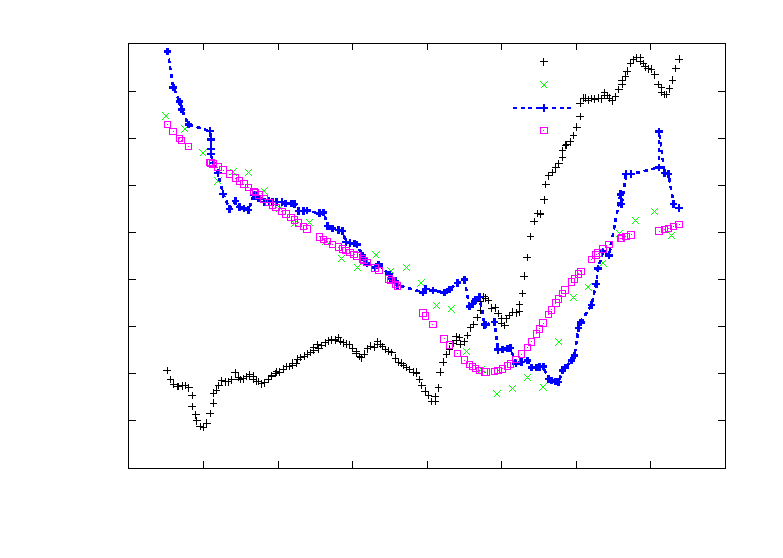
\includegraphics{../presentation/ekf_plot}}%
    \gplfronttext
  \end{picture}%
\endgroup
}
        \onslide<2>
        \vspace{-5cm}
        \begin{itemize}
            \item Implemented using \verb|robot_localization| ROS package
            \item Needs a great deal more tuning, but fusion is still better than discrete jumps
        \end{itemize}
    \end{overlayarea}
\end{frame}
}

\begin{frame}{Transformation Tree}
    \begin{columns}
        \begin{column}{0.4\textwidth}
            \begin{itemize}
                \item Maintain a tree of transformations (tfs) at all times
                \item Can lookup tf from any frame to any other...
                \item ... as long as they share some common node
            \end{itemize}
        \end{column}
        \begin{column}{0.6\textwidth}
            \includedot[scale=0.40]{../tikz/tf_frames}
        \end{column}
    \end{columns}
\end{frame}

\begin{frame}{Membership Functions}
    \centering
    \vspace{1em}
    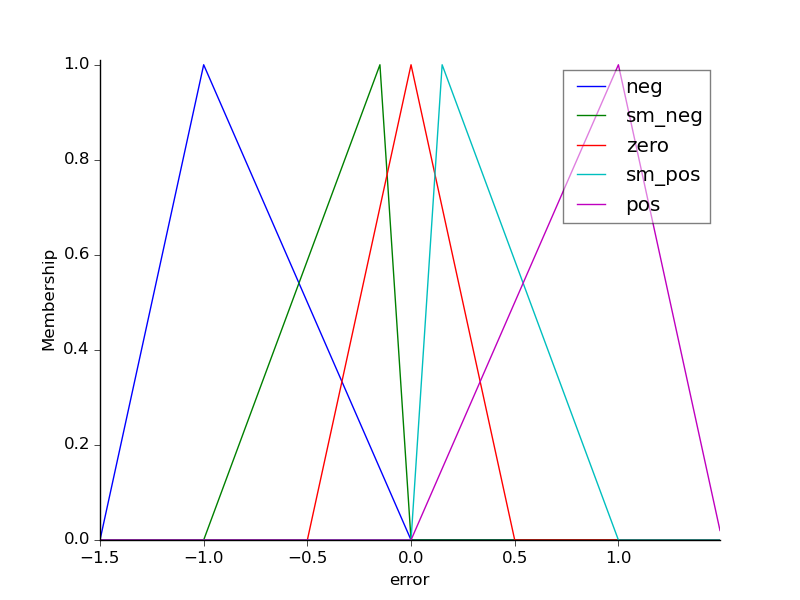
\includegraphics[width=0.45\textwidth]{../images/error_in.png}
    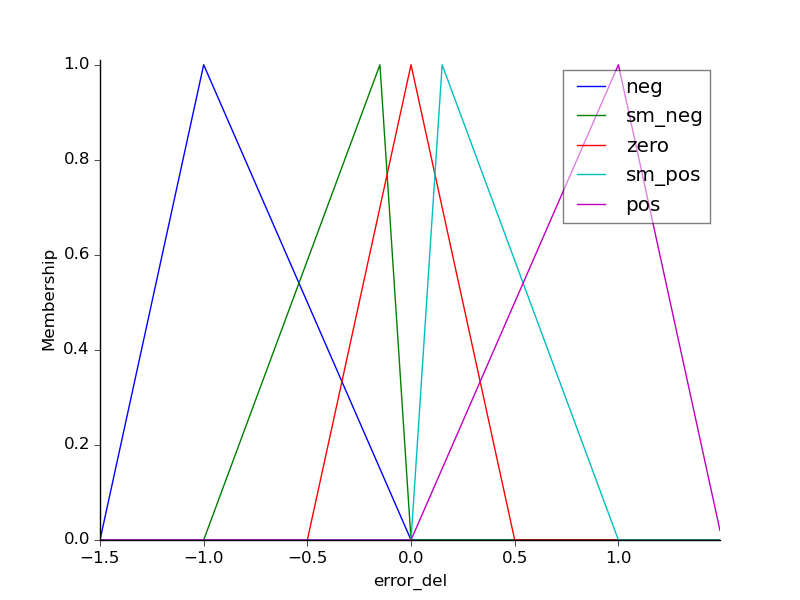
\includegraphics[width=0.45\textwidth]{../images/error_del_in.png}\\
    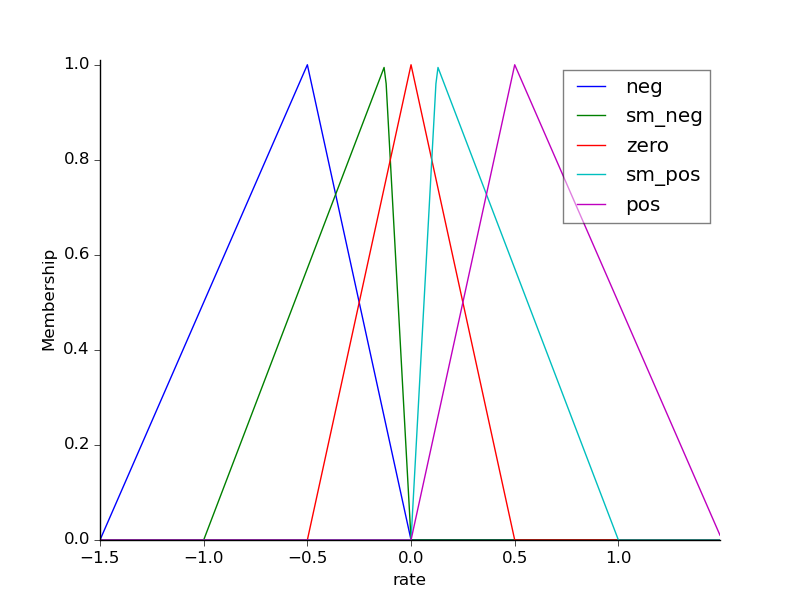
\includegraphics[width=0.45\textwidth]{../images/vel_out.png}
\end{frame}

\begin{frame}[fragile]{Rule Base}
%\begin{table}[ht]
    \centering
    %\caption{Fuzzy rule base}\label{t:rules}
    \hspace{3em}
    \begin{tabular}{cc||c|c|c|c|c|}
        &  \multicolumn{6}{c}{error}  \\ 	
        \multirow{6}{*}{error rate} &    & N  & SN & Z  & SP & P  \\ 	\hhline{~=#=|=|=|=|=|}
                                    & N  & P  & P  & SP & SP & Z  \\ 	\cline{2-7}
                                    & SN & P  & SP & SP & Z  & SN \\ 	\cline{2-7}
                                    & Z  & SP & SP & Z  & SN & SN \\ 	\cline{2-7}
                                    & SP & SP & Z  & SN & SN & N  \\ 	\cline{2-7}
                                    & P  & Z  & SN & SN & N  & N  \\ 	\cline{2-7}
                                    & \multicolumn{5}{c}{\hspace{4em}velocity}\\
    \end{tabular}
%\end{table}
\end{frame}

\section{Results}
\begin{frame}[fragile]{Static Target}
    \centering
    \vspace{1em}\hspace{3em}
    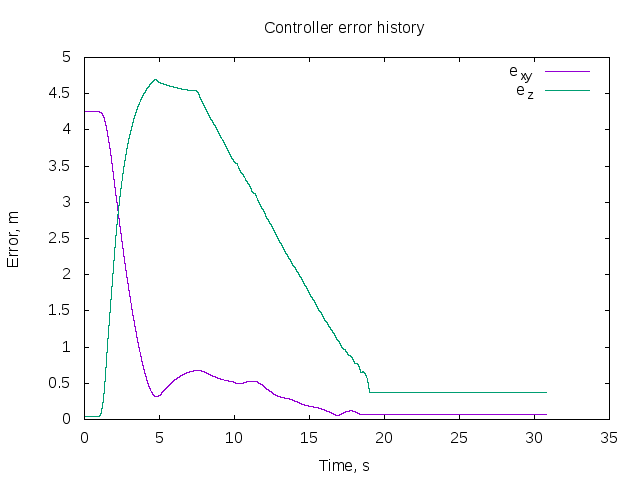
\includegraphics[width=0.8\textwidth]{../tikz/static_smach_good_plot}
\end{frame}

\fullFrameMovie{static_smach_good.mp4}{static_smach_good.jpg}

\begin{frame}{Moving Target}
    \centering
    \vspace{1em}\hspace{3em}
    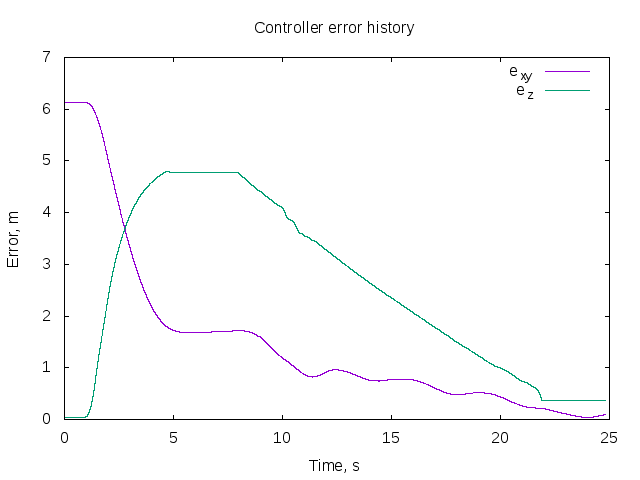
\includegraphics[width=0.8\textwidth]{../tikz/moving_line_good_plot}
    %\scalebox{0.8}{% GNUPLOT: LaTeX picture with Postscript
\begingroup
  \makeatletter
  \providecommand\color[2][]{%
    \GenericError{(gnuplot) \space\space\space\@spaces}{%
      Package color not loaded in conjunction with
      terminal option `colourtext'%
    }{See the gnuplot documentation for explanation.%
    }{Either use 'blacktext' in gnuplot or load the package
      color.sty in LaTeX.}%
    \renewcommand\color[2][]{}%
  }%
  \providecommand\includegraphics[2][]{%
    \GenericError{(gnuplot) \space\space\space\@spaces}{%
      Package graphicx or graphics not loaded%
    }{See the gnuplot documentation for explanation.%
    }{The gnuplot epslatex terminal needs graphicx.sty or graphics.sty.}%
    \renewcommand\includegraphics[2][]{}%
  }%
  \providecommand\rotatebox[2]{#2}%
  \@ifundefined{ifGPcolor}{%
    \newif\ifGPcolor
    \GPcolortrue
  }{}%
  \@ifundefined{ifGPblacktext}{%
    \newif\ifGPblacktext
    \GPblacktexttrue
  }{}%
  % define a \g@addto@macro without @ in the name:
  \let\gplgaddtomacro\g@addto@macro
  % define empty templates for all commands taking text:
  \gdef\gplbacktext{}%
  \gdef\gplfronttext{}%
  \makeatother
  \ifGPblacktext
    % no textcolor at all
    \def\colorrgb#1{}%
    \def\colorgray#1{}%
  \else
    % gray or color?
    \ifGPcolor
      \def\colorrgb#1{\color[rgb]{#1}}%
      \def\colorgray#1{\color[gray]{#1}}%
      \expandafter\def\csname LTw\endcsname{\color{white}}%
      \expandafter\def\csname LTb\endcsname{\color{black}}%
      \expandafter\def\csname LTa\endcsname{\color{black}}%
      \expandafter\def\csname LT0\endcsname{\color[rgb]{1,0,0}}%
      \expandafter\def\csname LT1\endcsname{\color[rgb]{0,1,0}}%
      \expandafter\def\csname LT2\endcsname{\color[rgb]{0,0,1}}%
      \expandafter\def\csname LT3\endcsname{\color[rgb]{1,0,1}}%
      \expandafter\def\csname LT4\endcsname{\color[rgb]{0,1,1}}%
      \expandafter\def\csname LT5\endcsname{\color[rgb]{1,1,0}}%
      \expandafter\def\csname LT6\endcsname{\color[rgb]{0,0,0}}%
      \expandafter\def\csname LT7\endcsname{\color[rgb]{1,0.3,0}}%
      \expandafter\def\csname LT8\endcsname{\color[rgb]{0.5,0.5,0.5}}%
    \else
      % gray
      \def\colorrgb#1{\color{black}}%
      \def\colorgray#1{\color[gray]{#1}}%
      \expandafter\def\csname LTw\endcsname{\color{white}}%
      \expandafter\def\csname LTb\endcsname{\color{black}}%
      \expandafter\def\csname LTa\endcsname{\color{black}}%
      \expandafter\def\csname LT0\endcsname{\color{black}}%
      \expandafter\def\csname LT1\endcsname{\color{black}}%
      \expandafter\def\csname LT2\endcsname{\color{black}}%
      \expandafter\def\csname LT3\endcsname{\color{black}}%
      \expandafter\def\csname LT4\endcsname{\color{black}}%
      \expandafter\def\csname LT5\endcsname{\color{black}}%
      \expandafter\def\csname LT6\endcsname{\color{black}}%
      \expandafter\def\csname LT7\endcsname{\color{black}}%
      \expandafter\def\csname LT8\endcsname{\color{black}}%
    \fi
  \fi
    \setlength{\unitlength}{0.0500bp}%
    \ifx\gptboxheight\undefined%
      \newlength{\gptboxheight}%
      \newlength{\gptboxwidth}%
      \newsavebox{\gptboxtext}%
    \fi%
    \setlength{\fboxrule}{0.5pt}%
    \setlength{\fboxsep}{1pt}%
\begin{picture}(7200.00,5040.00)%
    \gplgaddtomacro\gplbacktext{%
      \csname LTb\endcsname%
      \put(330,440){\makebox(0,0)[r]{\strut{}$0$}}%
      \put(330,1003){\makebox(0,0)[r]{\strut{}$1$}}%
      \put(330,1565){\makebox(0,0)[r]{\strut{}$2$}}%
      \put(330,2128){\makebox(0,0)[r]{\strut{}$3$}}%
      \put(330,2691){\makebox(0,0)[r]{\strut{}$4$}}%
      \put(330,3254){\makebox(0,0)[r]{\strut{}$5$}}%
      \put(330,3816){\makebox(0,0)[r]{\strut{}$6$}}%
      \put(330,4379){\makebox(0,0)[r]{\strut{}$7$}}%
      \put(462,220){\makebox(0,0){\strut{}$0$}}%
      \put(1730,220){\makebox(0,0){\strut{}$5$}}%
      \put(2998,220){\makebox(0,0){\strut{}$10$}}%
      \put(4267,220){\makebox(0,0){\strut{}$15$}}%
      \put(5535,220){\makebox(0,0){\strut{}$20$}}%
      \put(6803,220){\makebox(0,0){\strut{}$25$}}%
    }%
    \gplgaddtomacro\gplfronttext{%
      \csname LTb\endcsname%
      \put(3632,4709){\makebox(0,0){\strut{}Planar error}}%
      \csname LTb\endcsname%
      \put(5816,4206){\makebox(0,0)[r]{\strut{}e_{xy}}}%
      \csname LTb\endcsname%
      \put(5816,3986){\makebox(0,0)[r]{\strut{}e_z}}%
    }%
    \gplbacktext
    \put(0,0){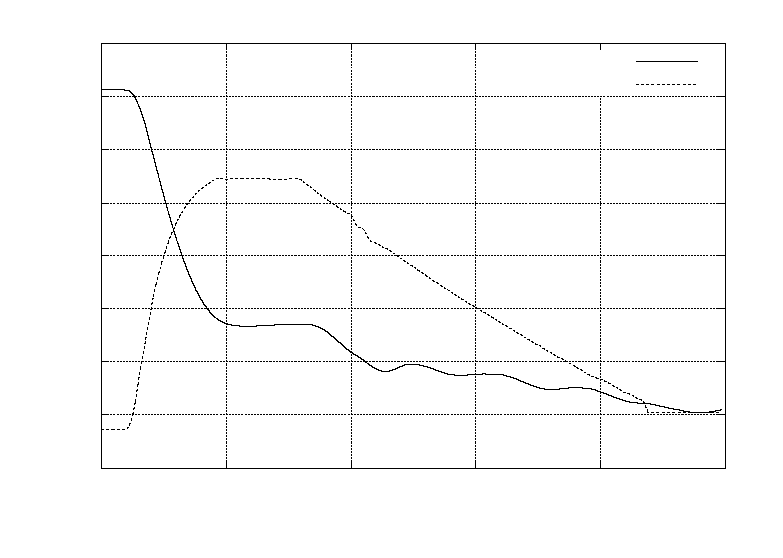
\includegraphics{moving_line_good_plot}}%
    \gplfronttext
  \end{picture}%
\endgroup
}
\end{frame}

\fullFrameMovie{moving_line_good.mp4}{moving_line_good.jpg}

\begin{frame}{Conclusions}
    \begin{itemize}
        \item Noisy data
        \item Different dynamic domains
        \item Comparable to gain-scheduled PID... without the need to schedule.
    \end{itemize}
\end{frame}

\begin{frame}{Future Work}
    \begin{itemize}
        \item Get it on hardware!
            \begin{itemize}
                \item MoCap functional
                \item EKF  tuning
                \item Brave soul
            \end{itemize}
        \item Send force/acceleration setpoints
            \begin{itemize}
                \item Not yet implemented in firmware
                \item Not trivial to add, but possible
            \end{itemize}
        \item Integrate with other tools like $\mathbbm{FlyMASTER}$ 
            \begin{itemize}
                \item Will make fuzzy control more accessible to others in the lab
                \item Both projects focused on modular control
                \item Recent work with capstone team proves possible
            \end{itemize}
    \end{itemize}
\end{frame}

\end{document}

